\section{Praktische Implementierung}

\subsection{Programmiersprache und Bibliotheken}
\subsubsection{Rust}
    Wie bereits im Abschnitt über verwandte Arbeiten angesprochen, sind wichtige Punkte bei der Implementierung von Algorithmen die 
    Geschwindigkeit und die Speichernutzung. Eine Programmiersprache, welche darauf ausgelegt ist in diesen Bereichen besonders effizient zu sein, 
    ist Rust. \cite{rust} Entworfen von Graydon Hoare, welcher seine Neuentwicklung im Juli 2010 das erste Mal  vorstellte, ist Rust eine sehr vielseitige Sprache.
    Mit dem Grundsatz einer open-source Multiparadigmen-Systemprogrammiersprache ist sie nicht nur für die breite Masse der Programmierer zugänglich, sondern auch 
    speziell für die Umsetzung von hardwarenaher Programmierung geeignet. Die Sprache setzt viele verschiedene Paradigmen der praktischen Programmierung um. So 
    unterstützt Rust sowohl funktionale als auch objektorientierte, sowie nebenläufige Programmierung. Auch ein hoher Abstraktionsgrad ist möglich. Vor allem aber 
    wurde beim Entwurf der Sprache darauf geachtet, dass die Kosten der Abstraktion zu Laufzeit so gering wie möglich sind. Man spricht von \emph{zero-cost-abstractions}, 
    welche beispielsweise auch bei der weitverbreiteten Programmiersprache \emph{C++} umgesetzt wurden. \cite{rust-wiki}
    Ein weiterer Vorteil von Rust ist, das die Sprache für \emph{cross-platform} Benutzung geeignet ist. Das bedeutet sie ist betriebssystemunabhängig. Das macht Rust zu einer 
    sehr einfach zugänglichen Sprache, da es nicht notwendig ist, ein UNIX-Basiertes- oder ein Windows-Betriebssystem zu besitzen oder gegebenenfalls ein Subsystem oder eine 
    Virtual Machine zu nutzen. All das würde zusätzlichen Aufwand bedeuten.
    Trotz allem sind natürlich, wie in keiner Programmiersprache, alle gewünschten Funktionen bereits implementiert. Bei Rust stellt das, durch den open-source Charakter,
    jedoch kein Problem dar. Die Community kann unter Nutzung des originalen Funktionsumfangs, der Standardbibliotheken, weitere neue Bibliotheken erstellen. 
    So ist beispielsweise die Bibliothek \emph{Iced} entstanden, welche für den Entwurf von \ac{gui}s gedacht ist. Im nächsten Kapitel ist darüber mehr zu lesen.
\subsubsection{Iced}
Wie bereits angedeutet, ist Iced eine Bibliothek für Rust, welche auf die Umsetzung von grafischen Nutzerinterfaces spezialisiert ist.
Der spanische Programmierer Héctor Ramón ließ sich bei Iced von der Sprache Elm inspirieren. Es ist zu erwähnen, dass sich Iced zum Zeitpunkt, da diese Arbeit verfasst wird, mit der Version 
0.4 noch im experimentellen Status befindet. Dennoch sind bereits die verschiedensten Funktionen nebst anschaulichen Beispielen für die Implementierung umgesetzt. Auch sind zwei verschiedene 
Renderer, also Software zum Darstellen von Grafiken auf dem Computerbildschirm, vorhanden. Namentlich \emph{iced-wgpu} und \emph{iced-glow}, unterstützt der erste der beiden die Verwendung von 
Vulkan \cite{vulkan}, Metal \cite{metal} und DirectX 12 \cite{dx12} und der zweite die Verwendung von OpenGL 2.1+ \cite{opgl} und OpenGL ES 2.0+ \cite{opgles}. \cite{iced}

\subsection{Entwurf des grafischen Nutzerinterfaces}
Eine Möglichkeit, um bereits in der Entwurfsphase auf Aspekte der Nutzerfreundlichkeit eingehen zu können, 
stellen Papierentwürfe dar. Dabei wird das \ac{gui}, statt aus digitalen Fenstern, aus einzelnen Blättern Papier gezeichnet und die Funktionen so simuliert. Dabei fallen negative Punkte wie zu tiefe oder breite 
Menüs auf und können direkt behoben werden, bevor sie schon im Code umgesetzt sind. Das vermeidet aufwendiges Umstrukturieren von hunderten Zeilen Code.

Bei dieser Arbeit gab es zwei konkurrierende Entwurfsideen, welche hier aus Gründen der Anschaulichkeit und Qualität nicht auf Papier dargestellt werden. Statt dessen werden digitale Skizzen verwendet, bei denen eventuelles Auffalten des Papiers
durch Pfeile und Beschriftung gekennzeichnet werden. 
Die Ideen unterscheiden sich vor allem durch das erste Menü, welches einmal die Optionen für die Triangulation inkludiert - im Folgenden als \emph{Menü Entwurf - Optionen inkludiert} und einmal ein Entwurf, bei dem 
die Optionen auf einem extra Menü nach Eingabe des Polygons aufgeführt werden. Dieser zweite Entwurf soll als \emph{Menü Entwurf - Optionen nachfolgend} bezeichnet werden.
Klar war jedoch von Beginn an, wie die Algorithmusiteration aussehen soll. Sie wird im Abschnitt \emph{Iteration Entwurf} dargestellt.
Zuletzt soll das Resultat des Algorithmus gezeigt werden. Auch hierfür gab es zwei unterschiedliche Konzepte. Einmal sollten zwei Anzeigen umgesetzt werden, zum einen das Ergebnis des gewählten Algorithmus und zum anderen das 
Ergebnis aus einer \ac{dt}, welche als optimales Ergebnis gilt und einen guten Qualitätsvergleich ermöglicht. Dieser Entwurf wird als \emph{Resultat Entwurf - Vergleichsfenster} bezeichnet.
Der andere Entwurf wird aufgrund der hier nur textlich dargestellten Metadaten als \emph{Resultat Entwurf - Metadaten} bezeichnet.


\subsubsection{Menü Entwurf - Optionen nachfolgend}
\raggedbottom
Dieser Entwurf sollte das Zeichen des Polygons in den Vordergrund stellen. Damit der Nutzer nicht von allen Optionen erschlagen wird, sondern diese nach und nach abarbeitet, wurden die Einstellungen in ein zweites Fenster 
ausgelagert. \pagebreak

\begin{figure}[t]
    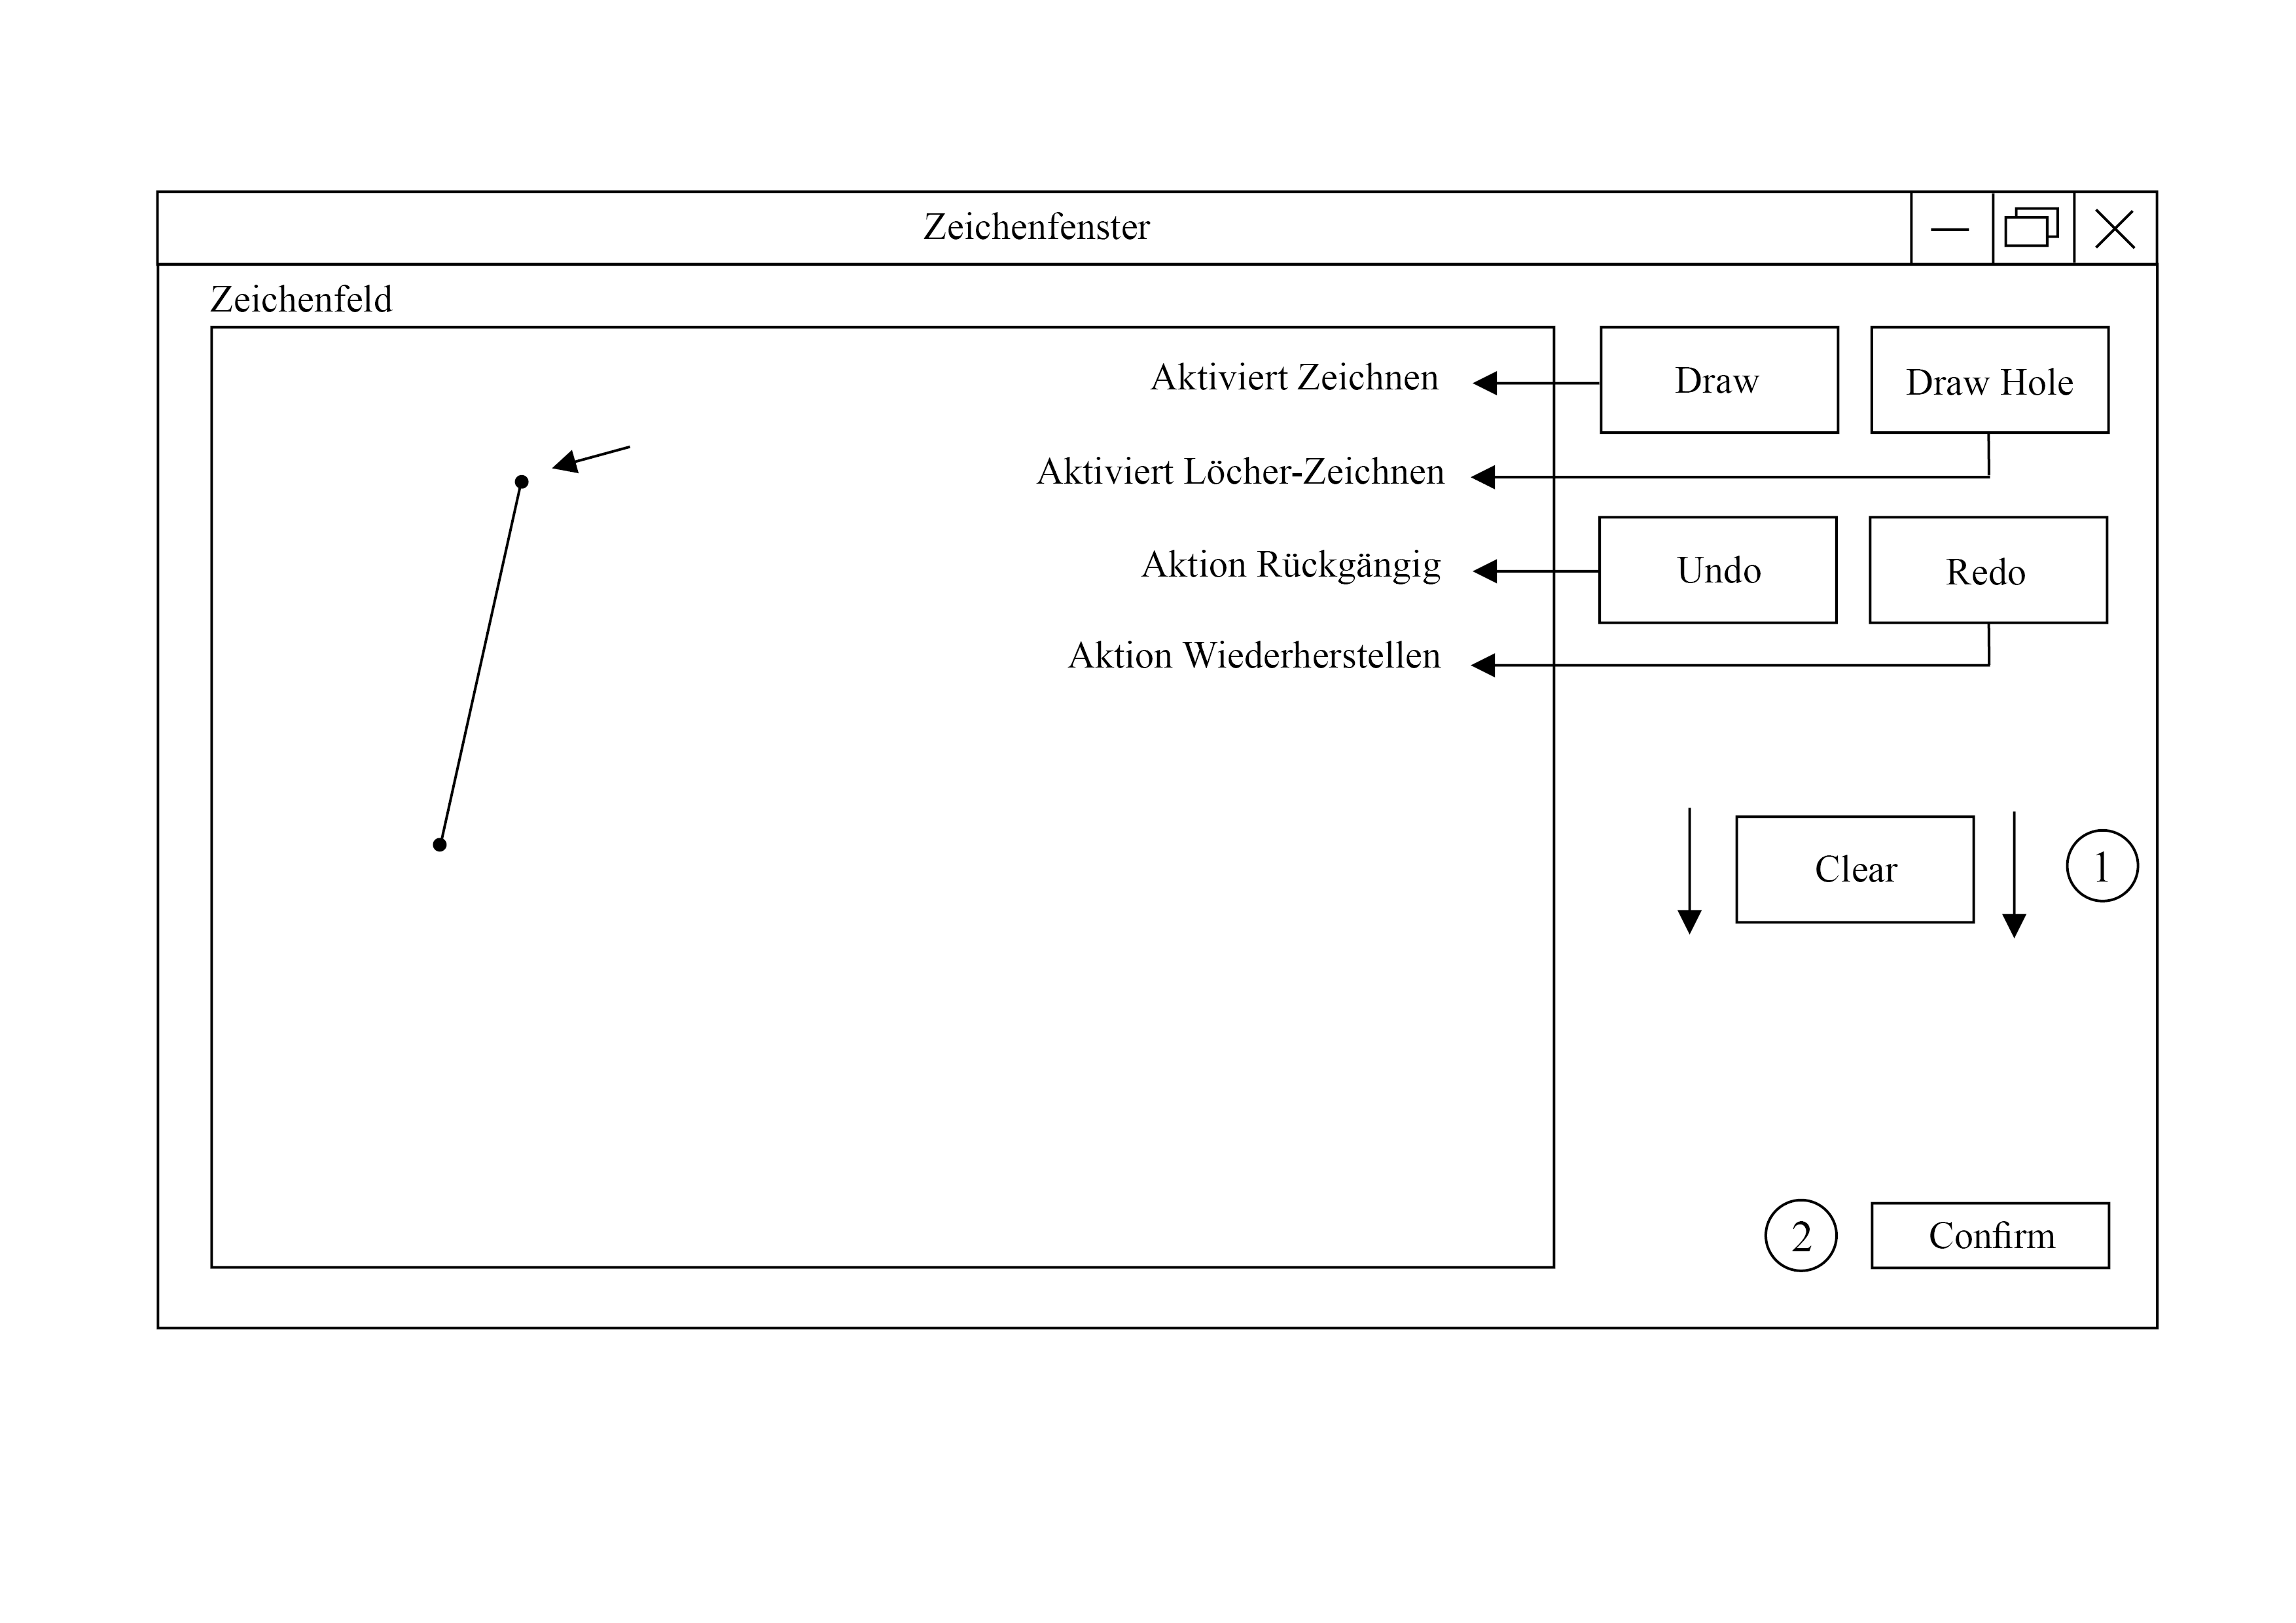
\includegraphics[width=0.9\textwidth]{bilder/menu_ohne_optionen.png}
    \caption[Entwurf des Menüs mit nachfolgenden Optionen]{Entwurf des Menüs mit nachfolgenden Optionen. links: Zeichenfeld für Eingabe des Polygons, rechts: Buttons mit Einfluss auf das Zeichenfenster. (1) öffnet Diaglogfenster (siehe Abbildung \ref{fig:cleardia})
    (2) Bestätigung des Polygons und Übergang in das Optionsfenster (siehe Abbildung \ref{fig:options})}
    \label{fig:menu_ohne_optionenen}
\end{figure}

Dieses erscheint nach Eingabe und Bestätigng des Poylgons durch Drücken auf den \emph{Confirm-Button}.(siehe Abbildung \ref{fig:options}) Dieser Fensterwechselt wurde mit der Nummer (2) gekennzeichnet. Die Buttons, welche sich alle in einer Box an der rechten Seite des Zeichenfeldes befinden, haben alle eine Funktion,
\begin{wrapfigure}{h}{0.6\textwidth}
    \centering
    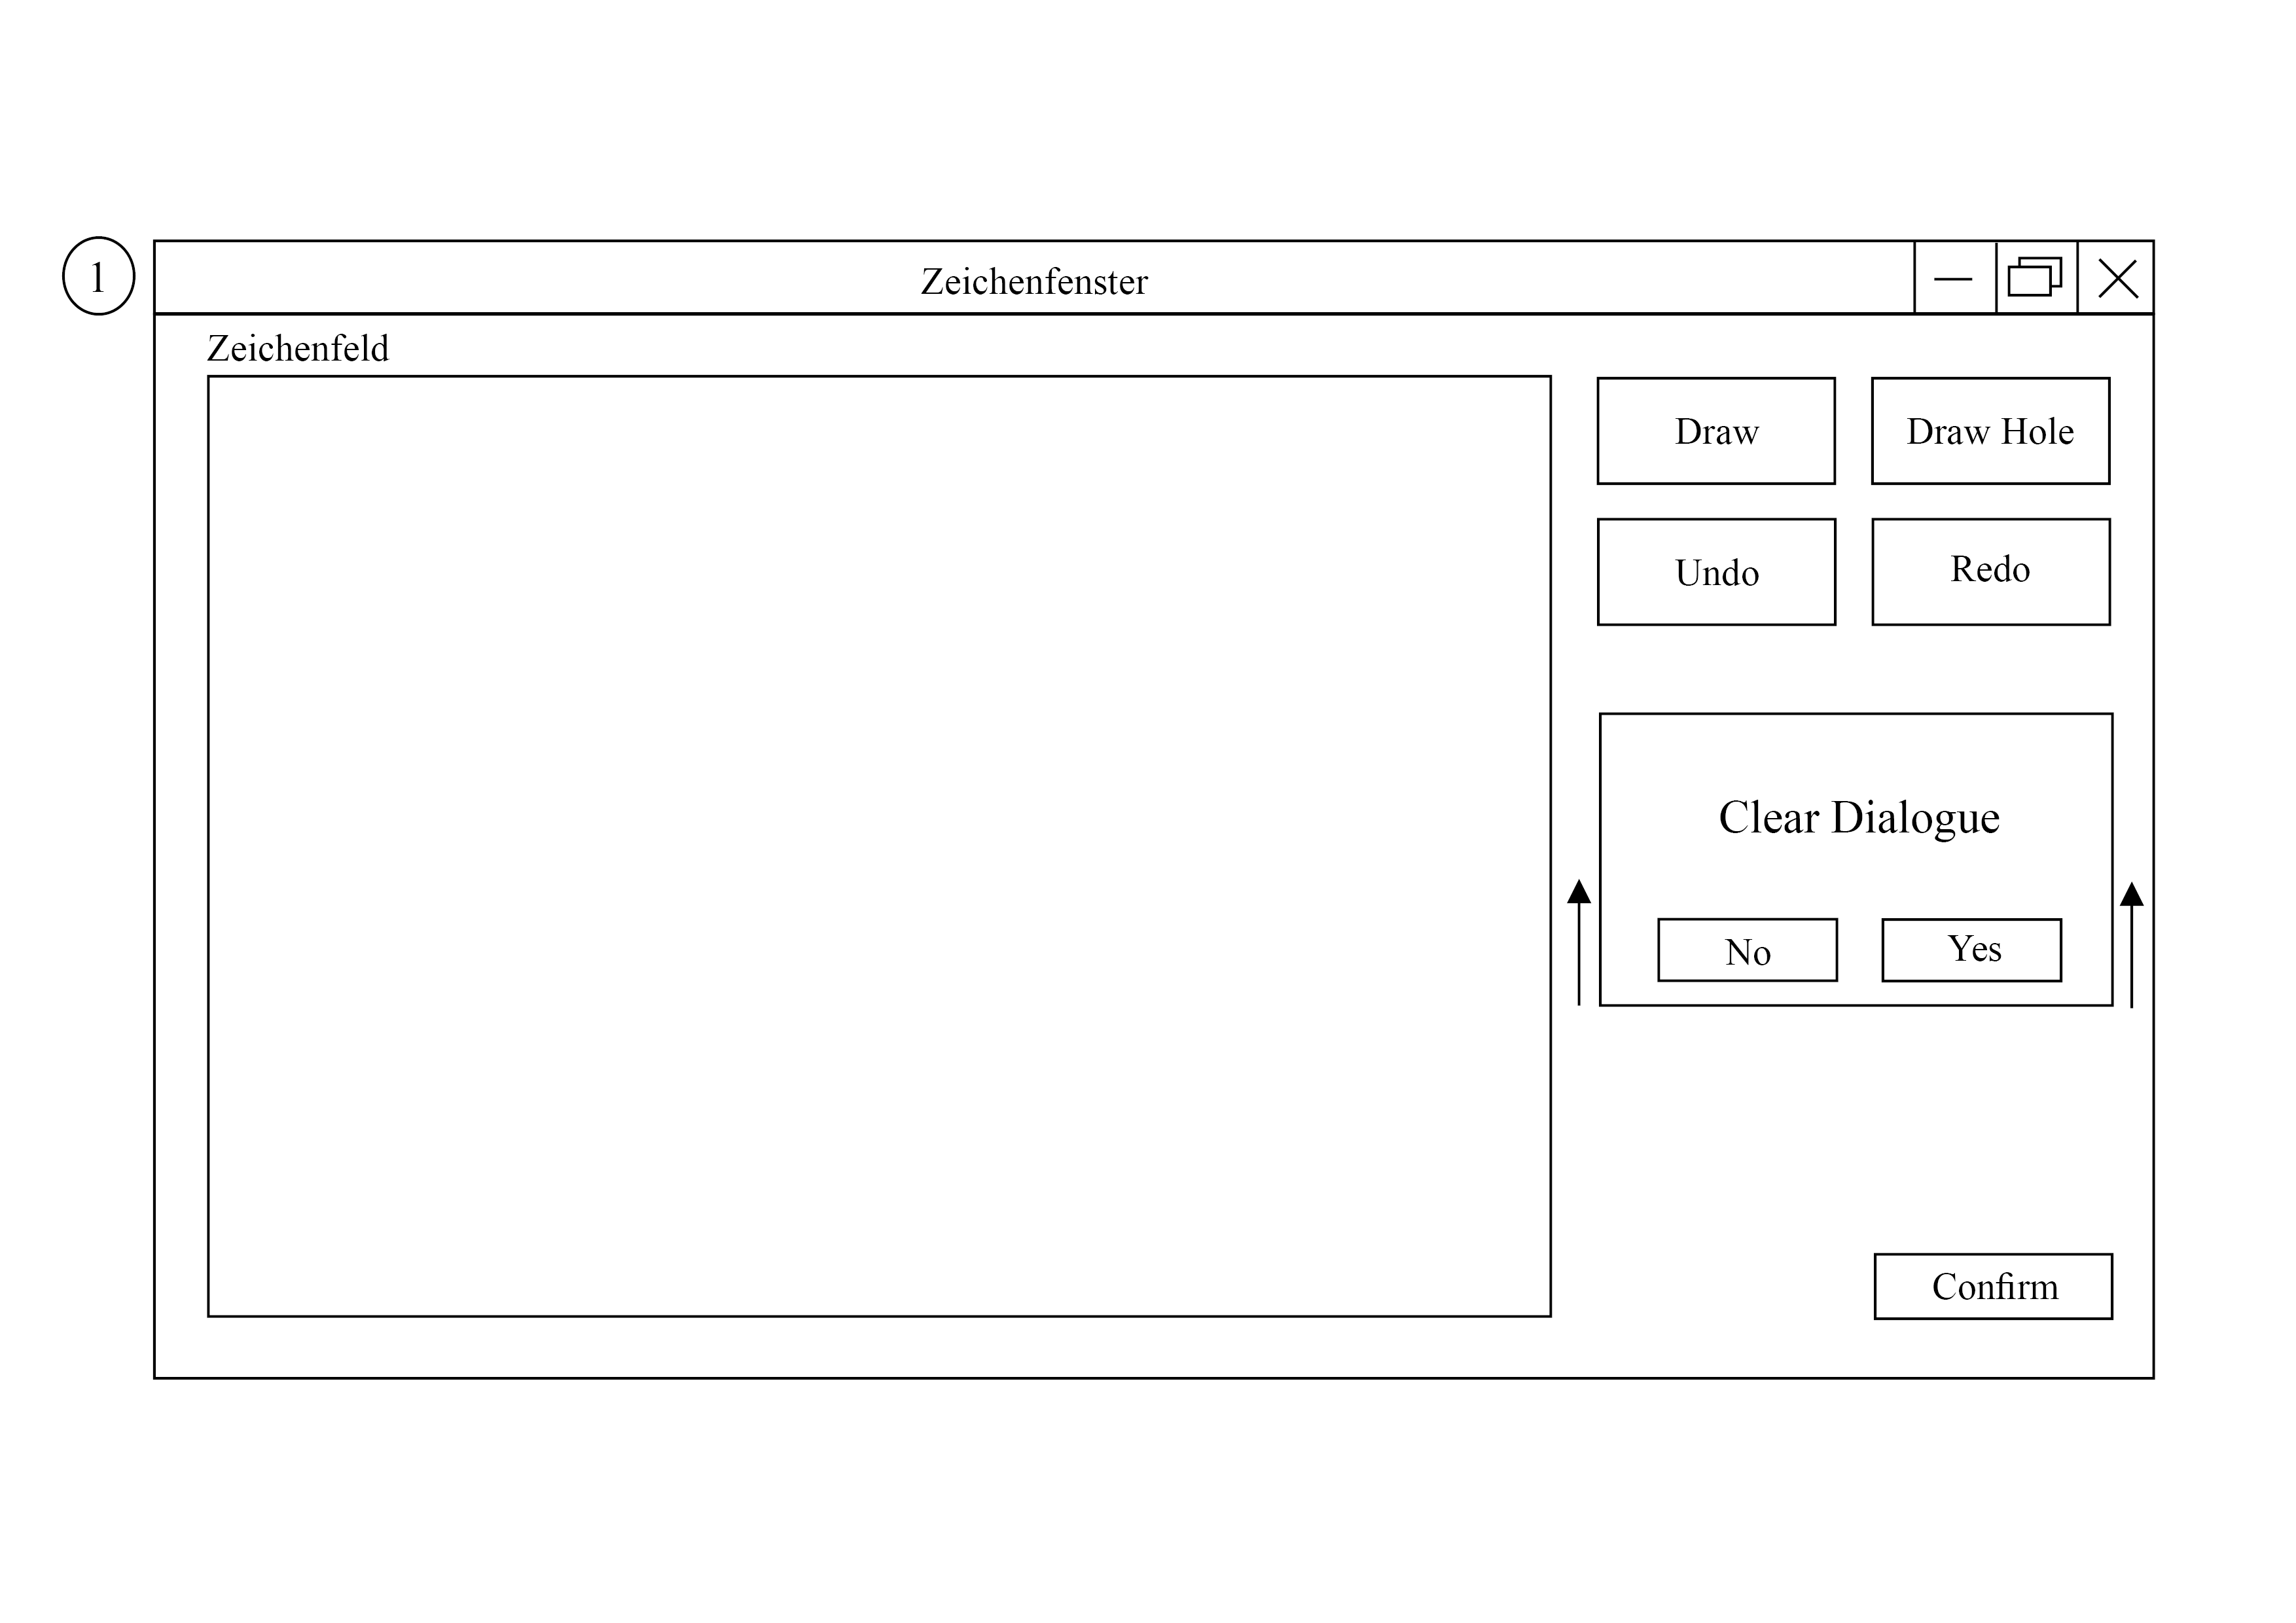
\includegraphics[width=0.6\textwidth]{bilder/cleardialogue.png}
    \caption[Öffnung des Dialogfensters]{Dialogfenster wurde durch bedienen des \emph{Clear-Buttons} aufgeklappt. Bestätigung oder Ablehnung durch den Nutzerw wird erwartet.}
    \label{fig:cleardia}
\end{wrapfigure}
welche das Zeichenfeld beeinflusst. 
Die Ausnahme ist hierbei der bereits angesprochene \emph{Confirm-Button}, welcher das eingegebene Polygon bestätigt und dann das Fenster mit den Optionen aufruft.
Der Einfluss der Buttons auf das Zeichenfenster ist mittels Pfeilen dargestellt, da sich augenscheinlich nichts am Aussehen des Fensters ändert.
Der \emph{Clear-Button} besitzt Pfeile nach unten. Dies soll den Übergang (1) andeuten. Dabei klappt ein Diaglogfenster an der Stelle dieses Buttons auf. Es ist dazu gedacht, um eine versehentliche Löschung aller Eingaben auf dem Zeichenfeld zu vermeiden.
Der Nutzer muss die Löschen-Aktion hier nocheinmal bewusst bestätigen. Wurde dieser Dialog beendet, dann klappt das Dialogfenster wieder zu und der  \emph{Confirm-Button} wird wieder sichtbar. Nachfolgend ist der Entwurf in digitaler Form zu sehen.    
    \begin{figure}[h]
        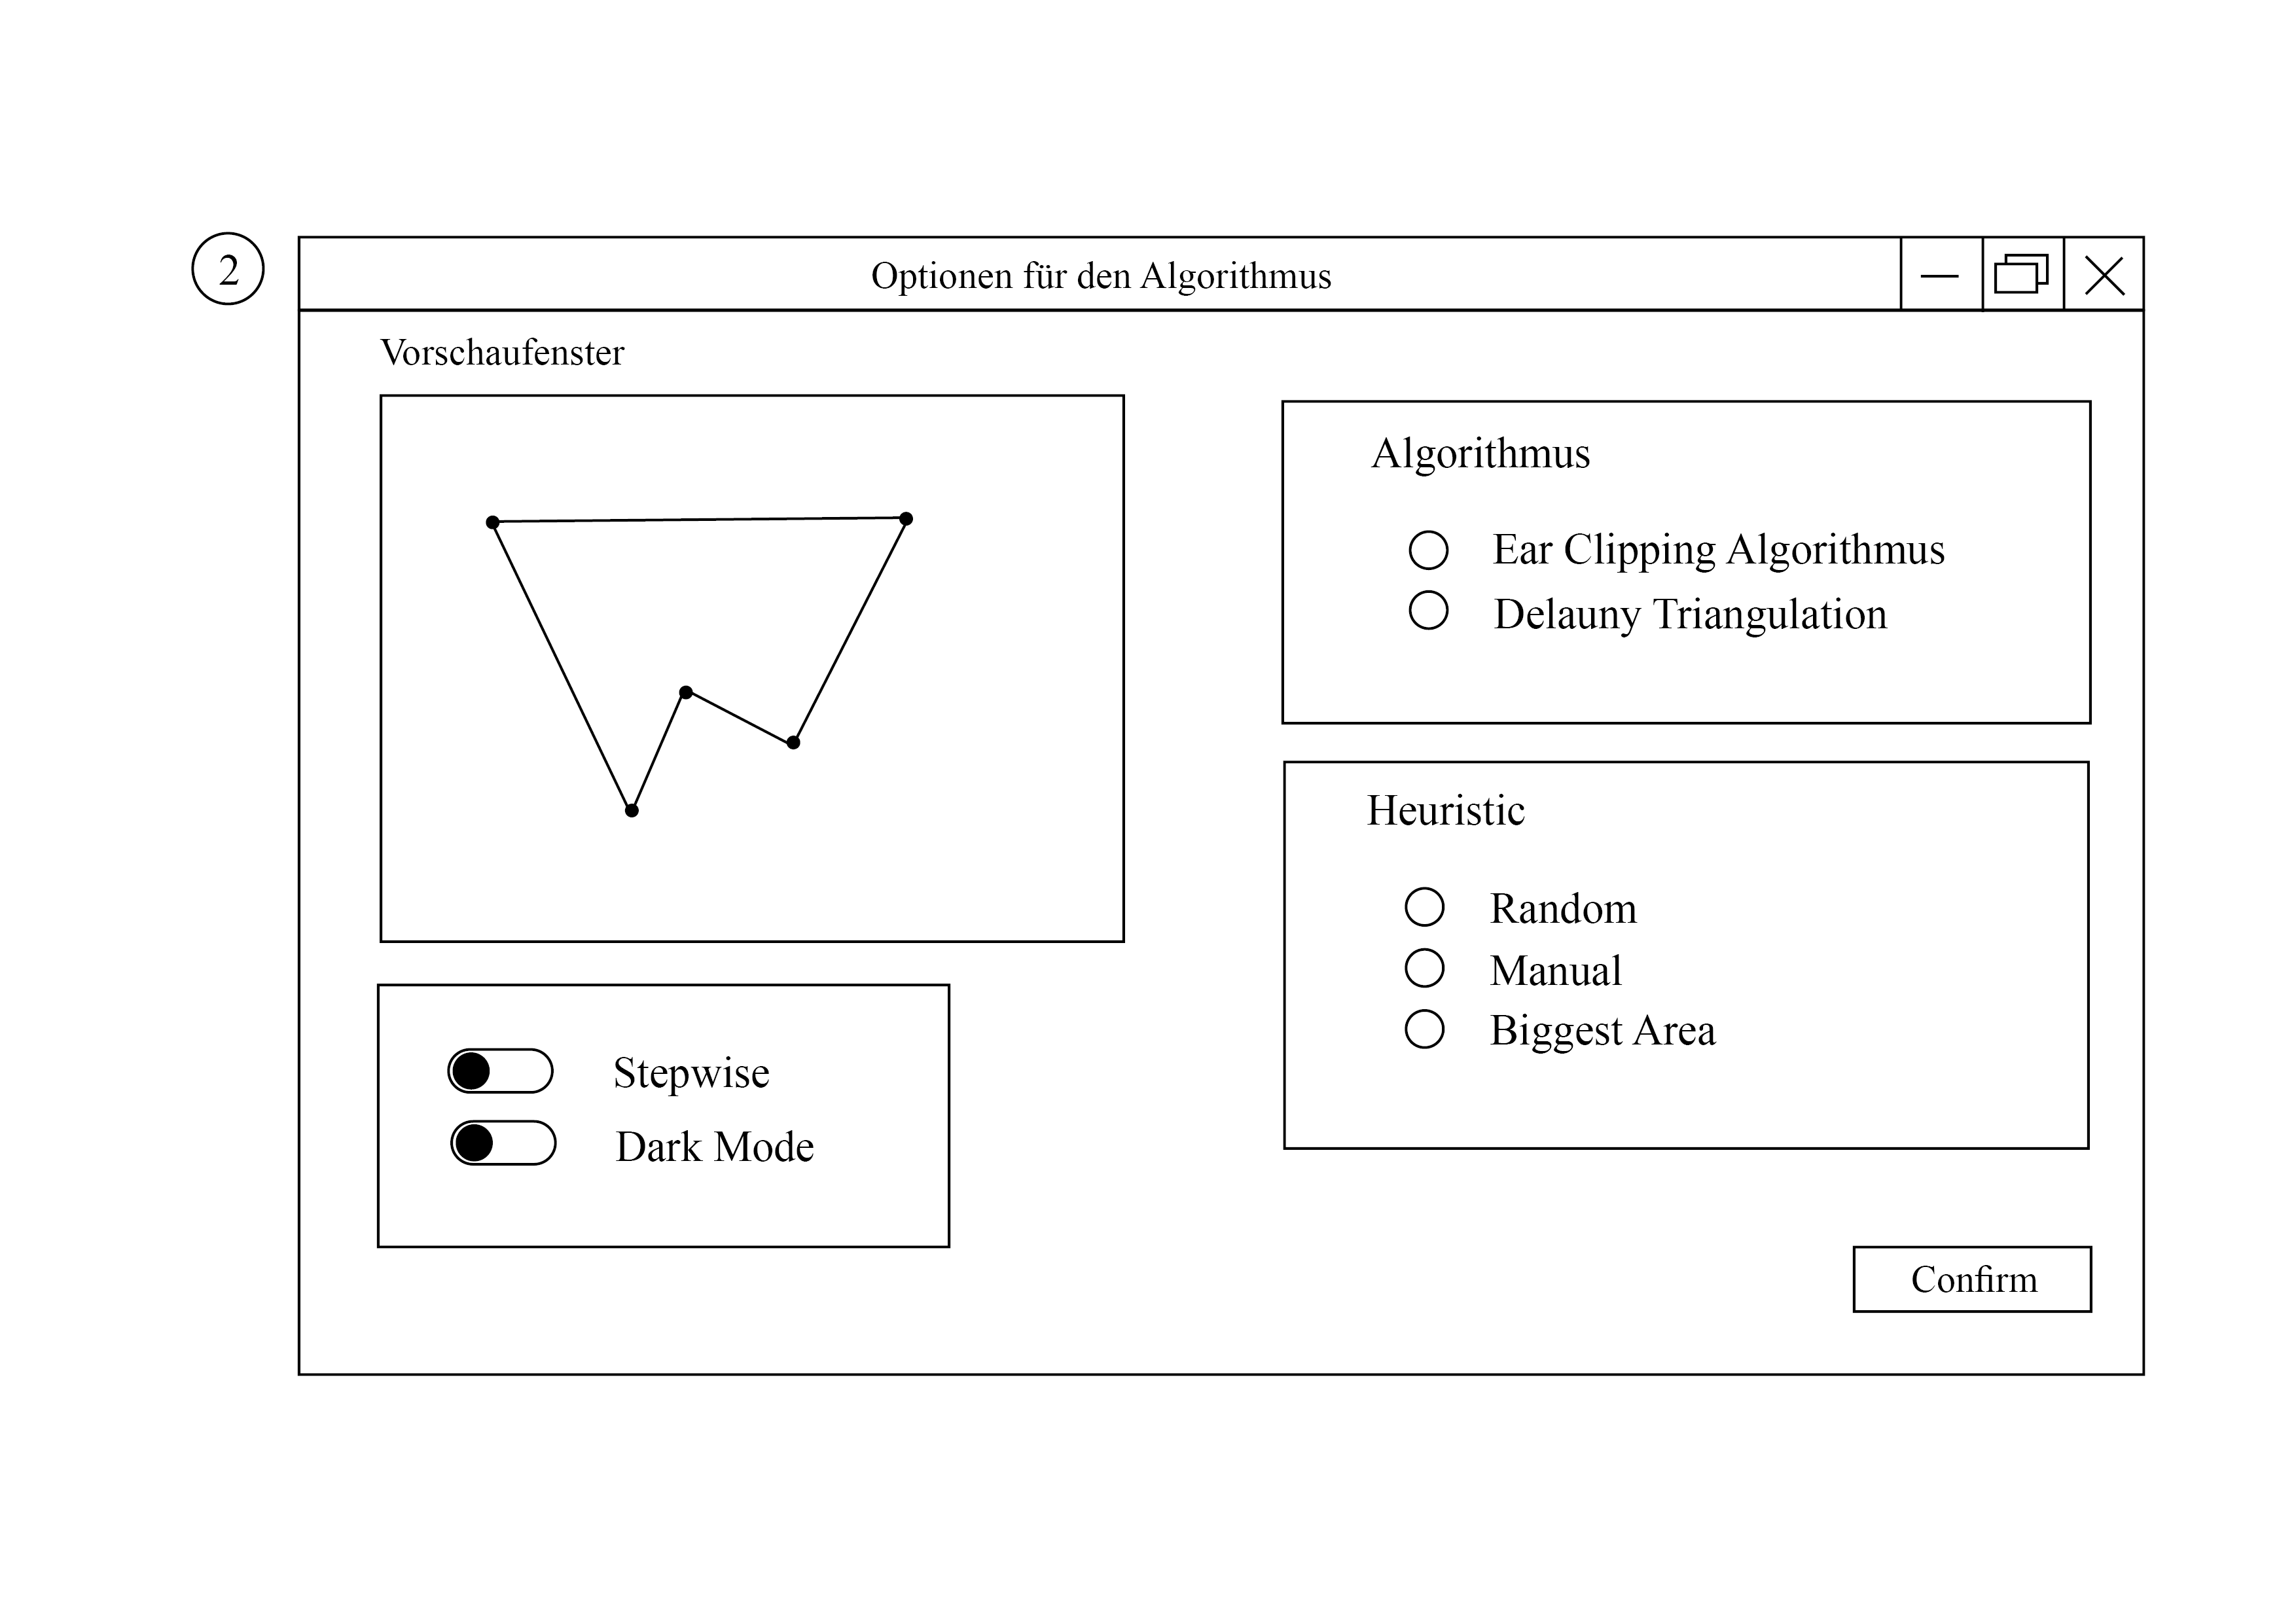
\includegraphics[width=1\textwidth]{bilder/optionsfenster.png}
        \caption[Ausgelagertes Optionsfenster]{Fenster, welches alle Optionen für den Algorithmus und die Software enthält. links: Vorschaufenster, darunter allgemeine Optionen. rechts: Algorithmus
        Auswahl und Auswahlt der Heuristik}
        \label{fig:options}
    \end{figure}

Wie in Abbildung \ref{fig:options} zu sehen ist, besteht das Optionsfentser aus vier Teilen. Oben links befindet sich das Vorschaufenster, welches das zuvor eingegebene Polygon zeigt. Es soll die gedankliche Verknüftung der Eingabe zu den Optionen herstellen.
Darunter befindet sich eine Gruppe von Togglern, welche die allgemeinen Optionen für die Ausführung des Algorithmus und das Aussehen der Anwendung beeinhalten.
Auf der rechten Seite befinden sich zwei Boxen, welche je eine Gruppierung von Radio Buttons umfassen. Die obere beinhaltet die Auswahl des Algorithmus. Die untere stellt die Auswahl der anzuwendenden Heuristik dar.
Durch einen weiteren \emph{Confirm-Button} wird der Übergang zur Iterationsseite geregelt.

Ein starker Nachteil dieses Entwurfs ist, dass alle Optionen, auch die allgemeinen, erst nach der ersten Eingabe zugänglich sind. Für das An- und Ausschalten des 
Dark Modes ist das unvorteilhaft. Auch sind nicht so viele Optionen vorhanden, dass der Nutzer überfordert werden könnte. 

Als vorteilhaft hingegen hat sich die Gruppierung der Buttons sowie der Radio Buttons erwiesen. Diese Unterstützung für den Nutzer, welche Bedienelemente zur selben Klasse gehören, stellte sich als positiv heraus.
Auch der Dialog zur Bestätigung des Löschens vermeidet eine Fehlbedienung und ist damit positiv zu bewerten.

\subsubsection{Menü Entwurf - Optionen inkludiert}
Der zweite Entwurf für das Menü beinhaltet auch die Optionen. Dies soll dem Nutzer alle Möglichkeiten auf einen Blick darbieten. Da es nicht sehr viele Auswahlmöglichkeiten gibt, sollte dieser Entwurf nicht zu Überforderung
des Benutzers führen. Im vorangegangenen Kapitell wurden einige Entwurfsstechniken angewendet, welche sich als vorteilhaft erwiesen. Hier sind zum Beispiel der Bestätigungsdialog und die Gruppierung ähnlicher Elemente zu nennen.
Diese wurden in diesen zweiten Entwurf übernommen. Auch bleibt das Zeichenfeld der größte Bereich des Menüs, um dieses in den Mittelpunkt der Anwendung zu stellen.

\begin{figure}[h]
    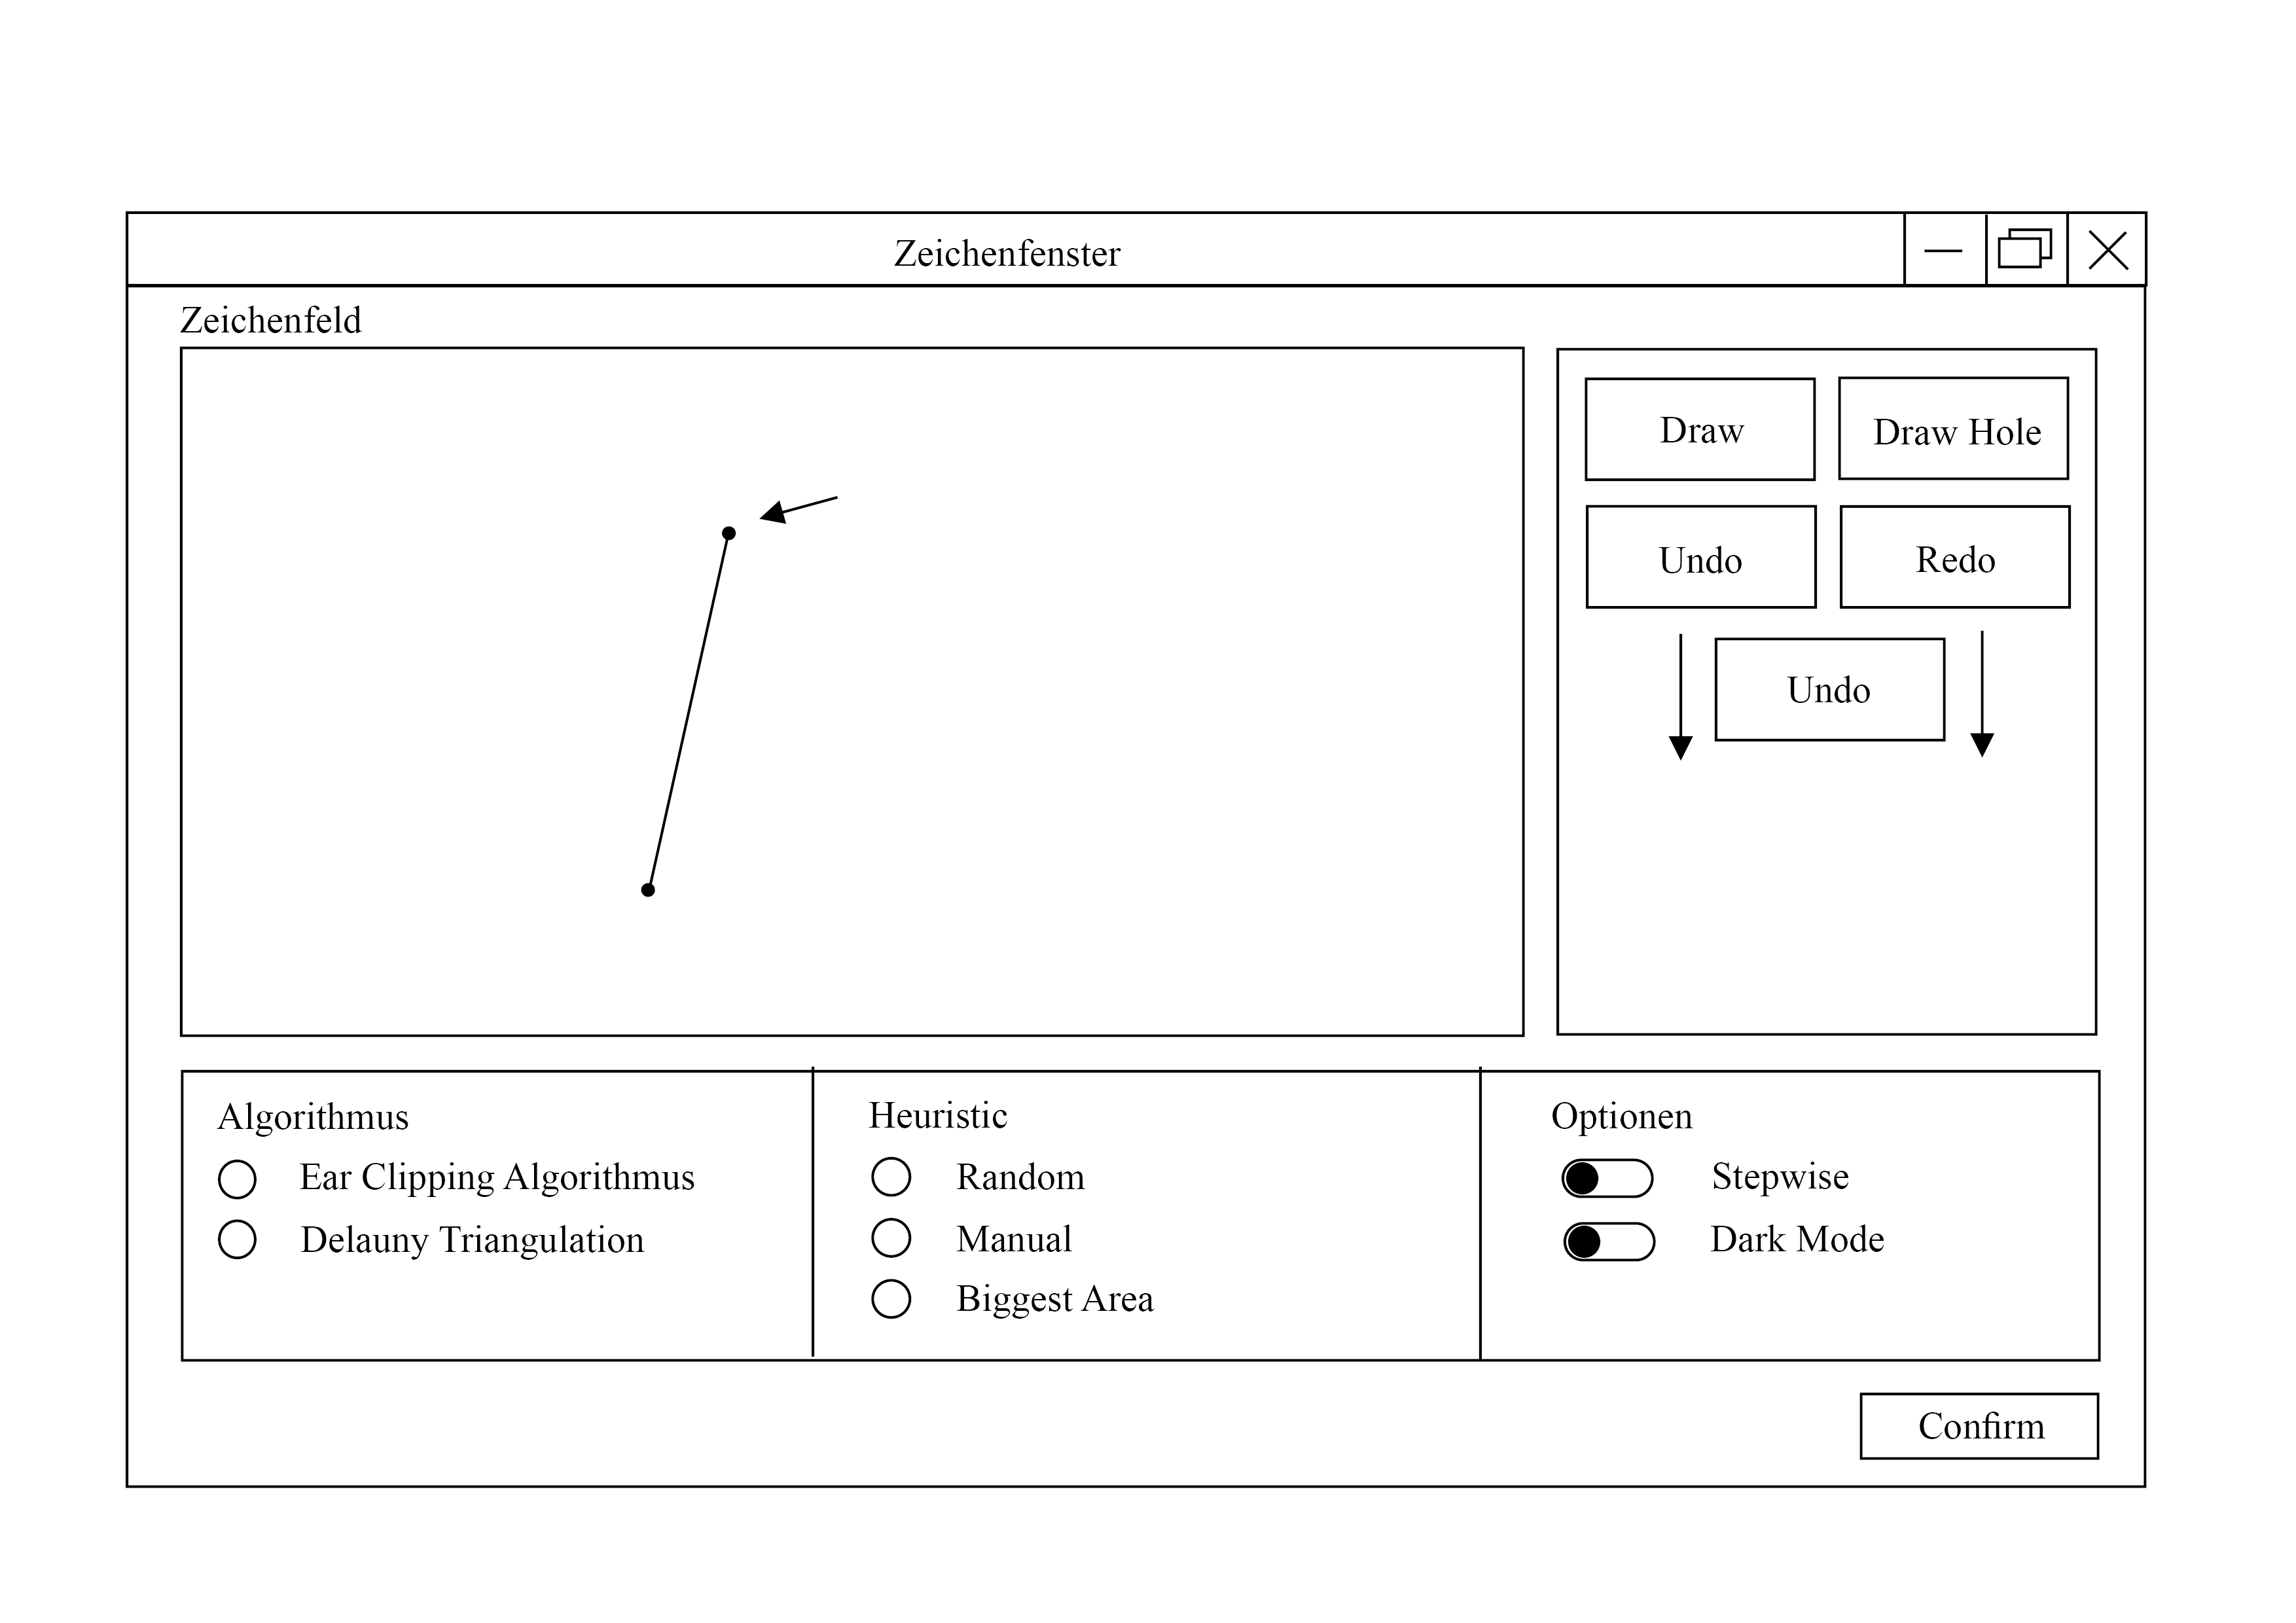
\includegraphics[width=1\textwidth]{bilder/menu_mit_optionen.png}
    \caption[Entwurf für das Menü mit Optionen]{Menü ähnlich dem Entwurf mit ausgelagerten Optionen. Hier im unteren Bereich drei Sektionen für die Einstellungsmöglichkeiten.}
    \label{fig:menu_mit_optionen}
\end{figure}

Wie in der Abbildung \ref{fig:menu_mit_optionen} zu sehen ist, wurde der \emph{Confirm-Button} aus der Gruppe der Zeichenwerkzeuge ausgelagert. Das hat den Grund, dass er nicht nur die Zeichnung sondern auch alle gewählten Optionen bestätigt.
Daher befindet er sich ganz unten rechts. Auch in den folgenden Entwürfen wird der Button für den Übergang zur nächsten Seite an dieser Stelle sein. Somit ist einen gewisse Einheitlichkeit gewährleistet.
Die nächste Seite, welche durch den \emph{Confirm-Button} aufgerufen wird, ist, anders als im vorangegangenen Entwurf, sofort die Iterationsseite, nicht eine weitere Seite mit Optionen.
Die anderen Funktionen der Buttons und Optionen wurden bereits in Kapitel 4.2.1 beschrieben und sollen daher nicht an dieser Stelle erneut thematisiert werden.

\subsubsection{Iteration Entwurf}
Die Iterationsseite bestitzt eine klar definierte Funktion. Sie soll den Algorithmus schrittweise darstellen. Dafür bedarf es lediglich weniger Interaktionselemente. 
Zu allererst wird ein Vorschaufenster benötigt. Dieses steht im Mittelpunkt und ist daher besonders groß. Darunter befindet sich links ein Button, welcher es ermöglicht, die Schritte rückwärts darzustellen. Das funktioniert allerdings nur,
solange mehr als ein Schritt druchlaufen wurde. In der Mitte des unteren Randes befindet sich eine Fortschrittsanzeige, welche die Rückkopplung zum Nutzer darstellt. Hier wird der aktuelle Schritt in Relation zur gesamten Schrittanzahl gezeigt.
Rechts davon befindet sich der \emph{Next-Button}. Wird dieser gedrückt, dann wird auf dem Vorschaufenster der nächste Iterationsschritt angezeigt und die Fortschrittsanzeige einen Zähler nach oben gestellt.
Sind alle Schritte abgearbeitet, dann wird über den \emph{Next-Button} die nächste Seite, die Ergebnisseite, aufgerufen.

\begin{figure}[h]
    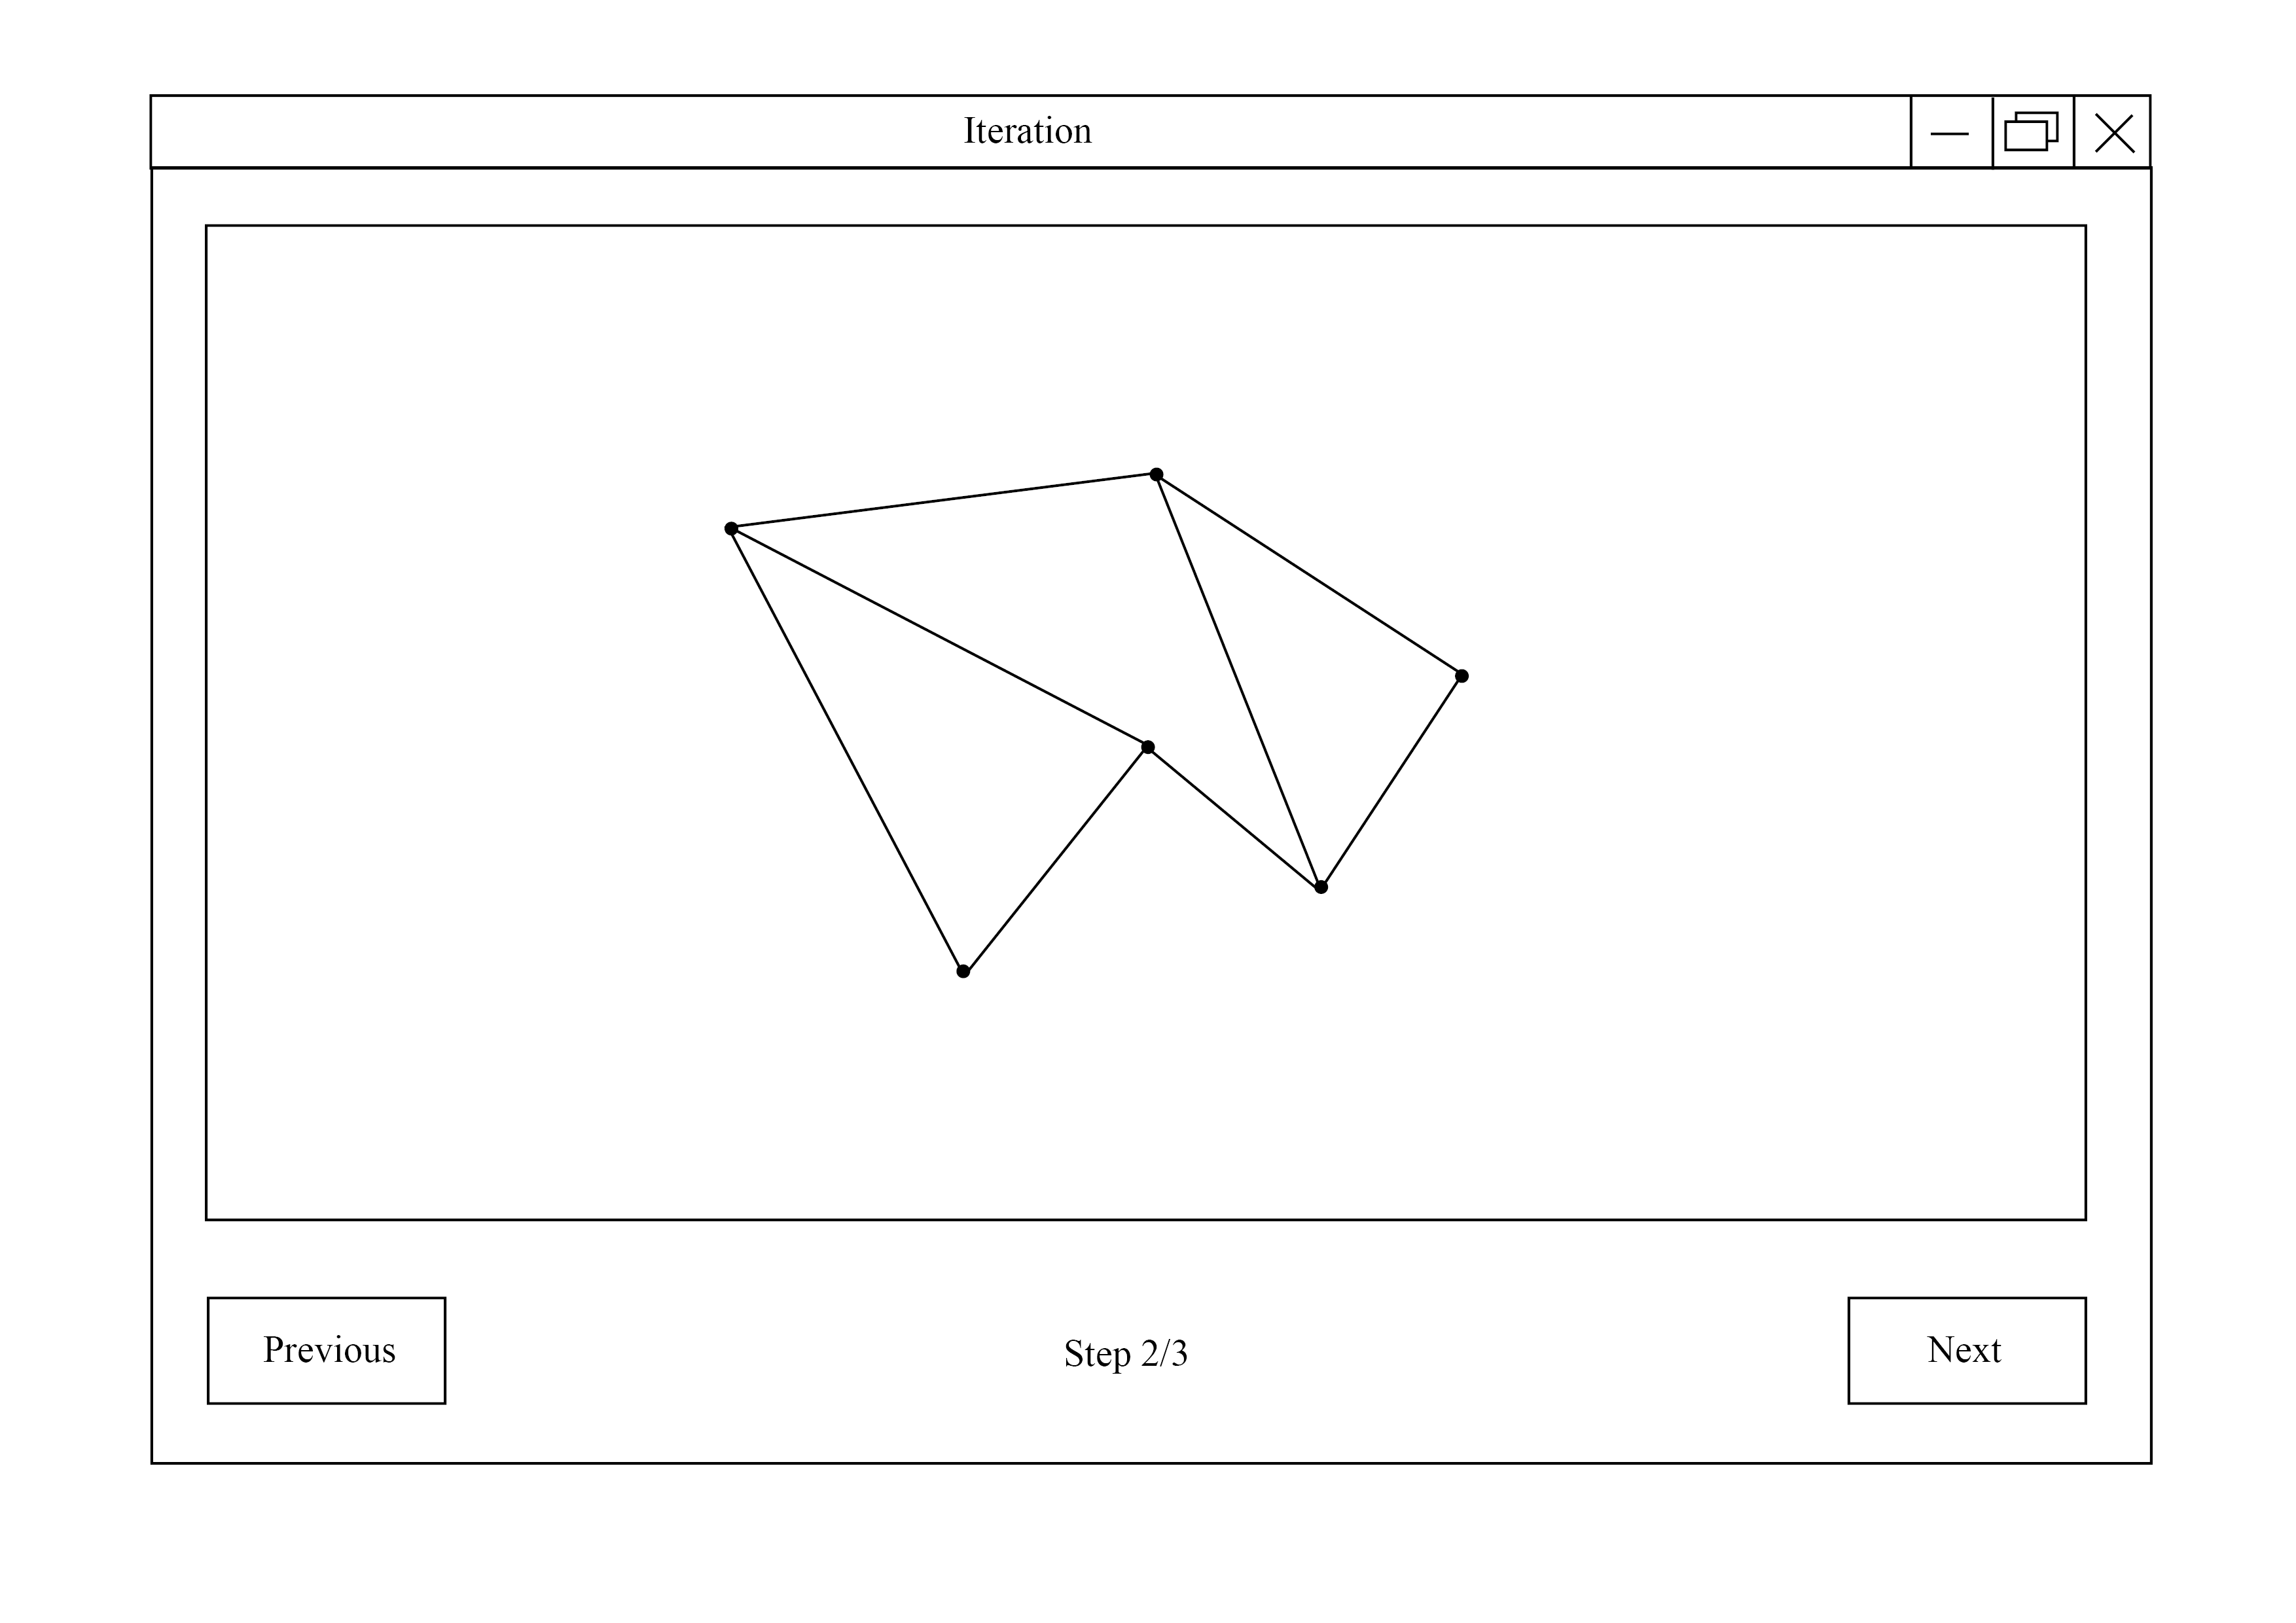
\includegraphics[width=1\textwidth]{bilder/iteration.png}
    \caption[Entwurf Iterationsseite]{Iterationsseite aus Vorschaufenster und Navigationsleiste mit Fortschrittsanzeige}
    \label{fig:iteration}
\end{figure}

Eine Entwurfsverbesserung, welche zu einem späteren Zeitpunkt aufkam, war, dass der \emph{Next-Button} nachdem der letzte Iterationsschritt durchgeführt wurde, seine Beschriftung auf \emph{End} wechselt.
Das soll beim Nutzer die Assoziation wecken, dass der Iterationsprozess abgeschlossen ist. Der Übergang auf die Ergebnisseite wird damit besser an den Anwender vermittelt.

\subsubsection{Resultat Entwurf - Metadaten}
Der erste Entwurf für die Ergebnisseite, auf welcher das Resultat der Algorithmusiteration zu sehen sein soll, umfasst wie die Iterationsseite nur drei Elemente.
Das Ergebnisfenster, welches das zerlegte Polygon zeigt, ist dabei fast seitenfüllend und damit das Zentrum der Betrachtung.
Darunter ist auf der linken Seite der \emph{Exit-Button}. Dieser beendet das Programm. Sein Gegenstück befindet sich auf der rechten Seite. Der \emph{Return-to-Menu-Button} (im Folgenden \emph{Return-Button})  
lässt den Nutzer, wie die Aufschrift bereits andeutet, auf die Menüseite zurückkehren. Dort wird das zuvor eingegebene Polygon im Zeichenfeld angezeigt. Es kann jetzt verändert werden. Auch können andere Einstellungen getroffen werden 
und der Algorithmus dann erneut durchgeführt werden.

Da allerings eine reine Anzeige des zerlegten Polygons wenig über seine Qualität aussagt, wurde dieser Entwurf noch angepasst. Unter dem Ergebnisfenster werden noch einige Daten über das Polygon und die Dreiecke dargestellt, welche die Zerlegung bilden.
Das sieht dann wie folgt aus:

\begin{figure}[h]
    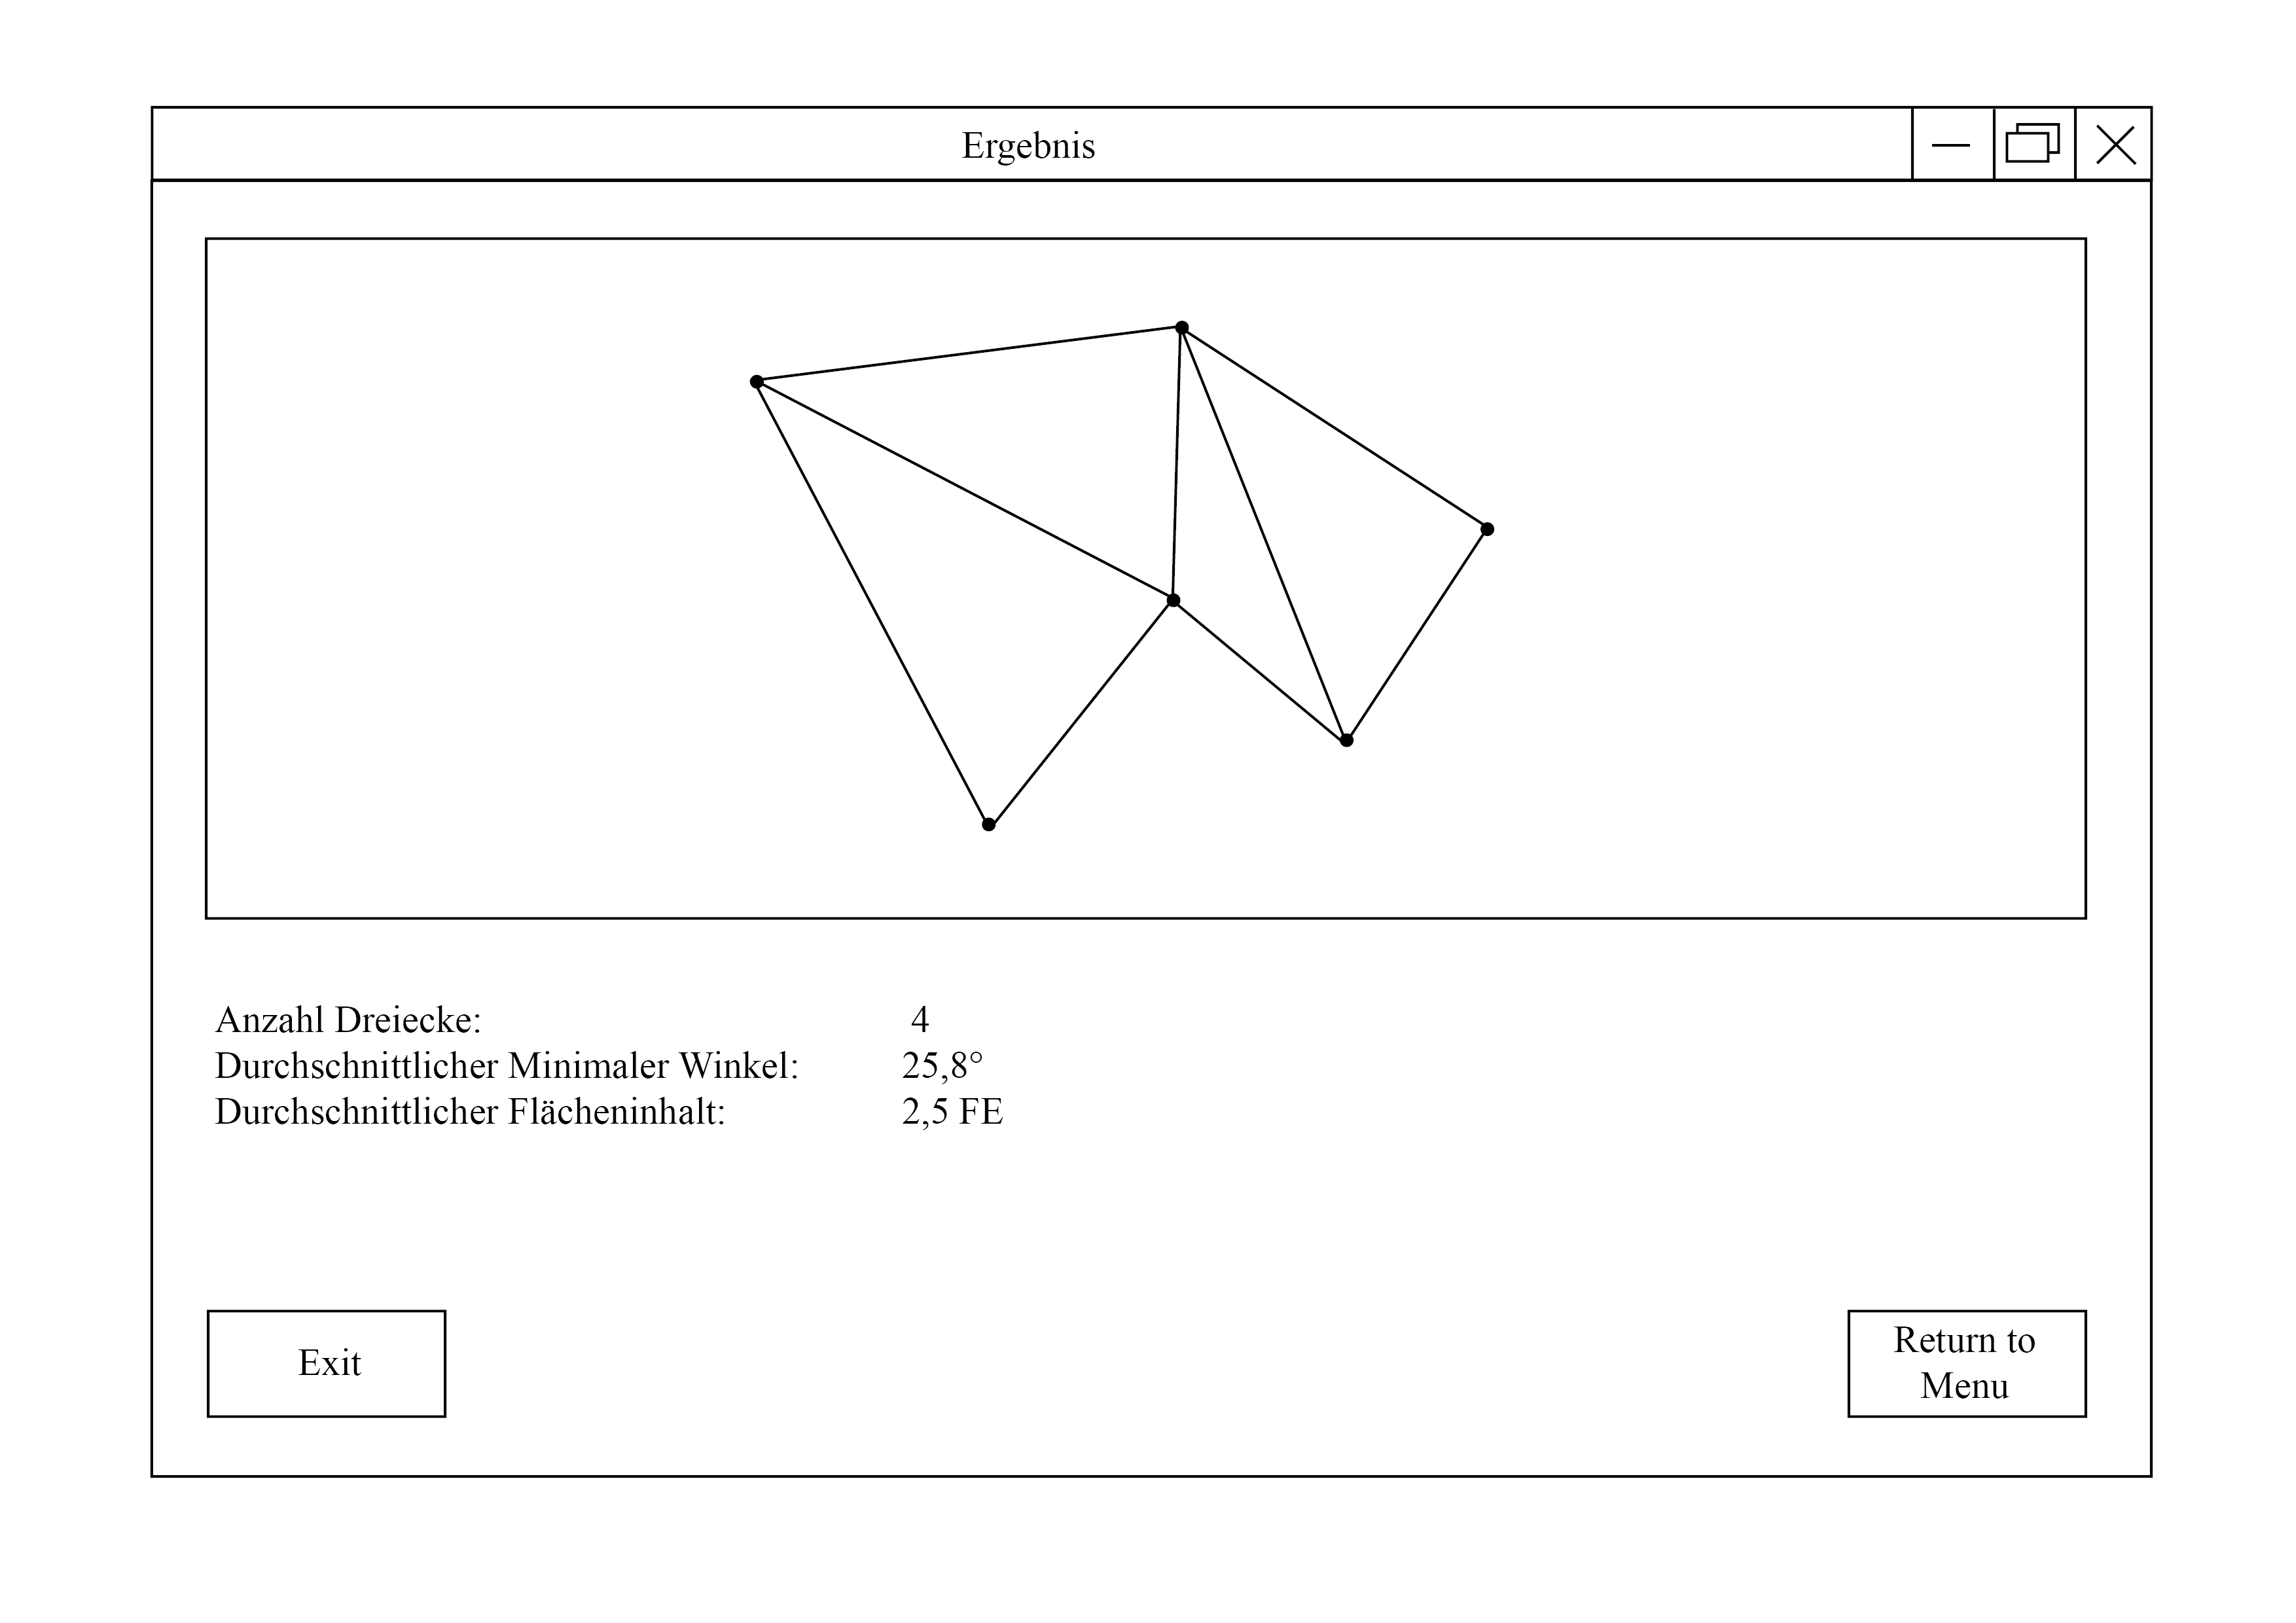
\includegraphics[width=1\textwidth]{bilder/ergebnis_metadaten.png}
    \caption[Entwurf Ergebnisseite mit Metadaten]{Ergebnisseite mit Ergebnisfenster und darunter Daten über das zerlegte Polygon}
    \label{fig:ergebnis_meta}
\end{figure}

\subsubsection{Resultat Entwurf - Vergleichsfenster}
Eine weitere Verbesserung der Ergebnisseite stellt dieser Entwurf dar. Zwar wurde der ursprüngliche Entwurf durch die Einführung der weiteren Informationen über das Polygon verbessert, jedoch fehlt immer noch eine Vergleichsmöglickeit.
Natürlich könnte der Nutzer mittels Bildschirmfoto und späterem Vergleich feststellen, welche seiner Einstellung die optimale Zerlegung herbeigeführt hat, jedoch ist das umständlich.
Um diesen Vergleich zu erleichtern, wird in diesem Entwurf ein zweites Anzeigefenster hinzugefügt. Dieses soll die perfekte Zerlegung des eingegebenen Polygons sowie seine Metadaten darstellen.
Damit kann der Nutzer feststellen, wie weit er vom Idealwert entfernt ist. Die übrigen Funktionen der Ergebnisseite werden aus dem vorangegangenen Entwurf übernommen.

\begin{figure}[h]
    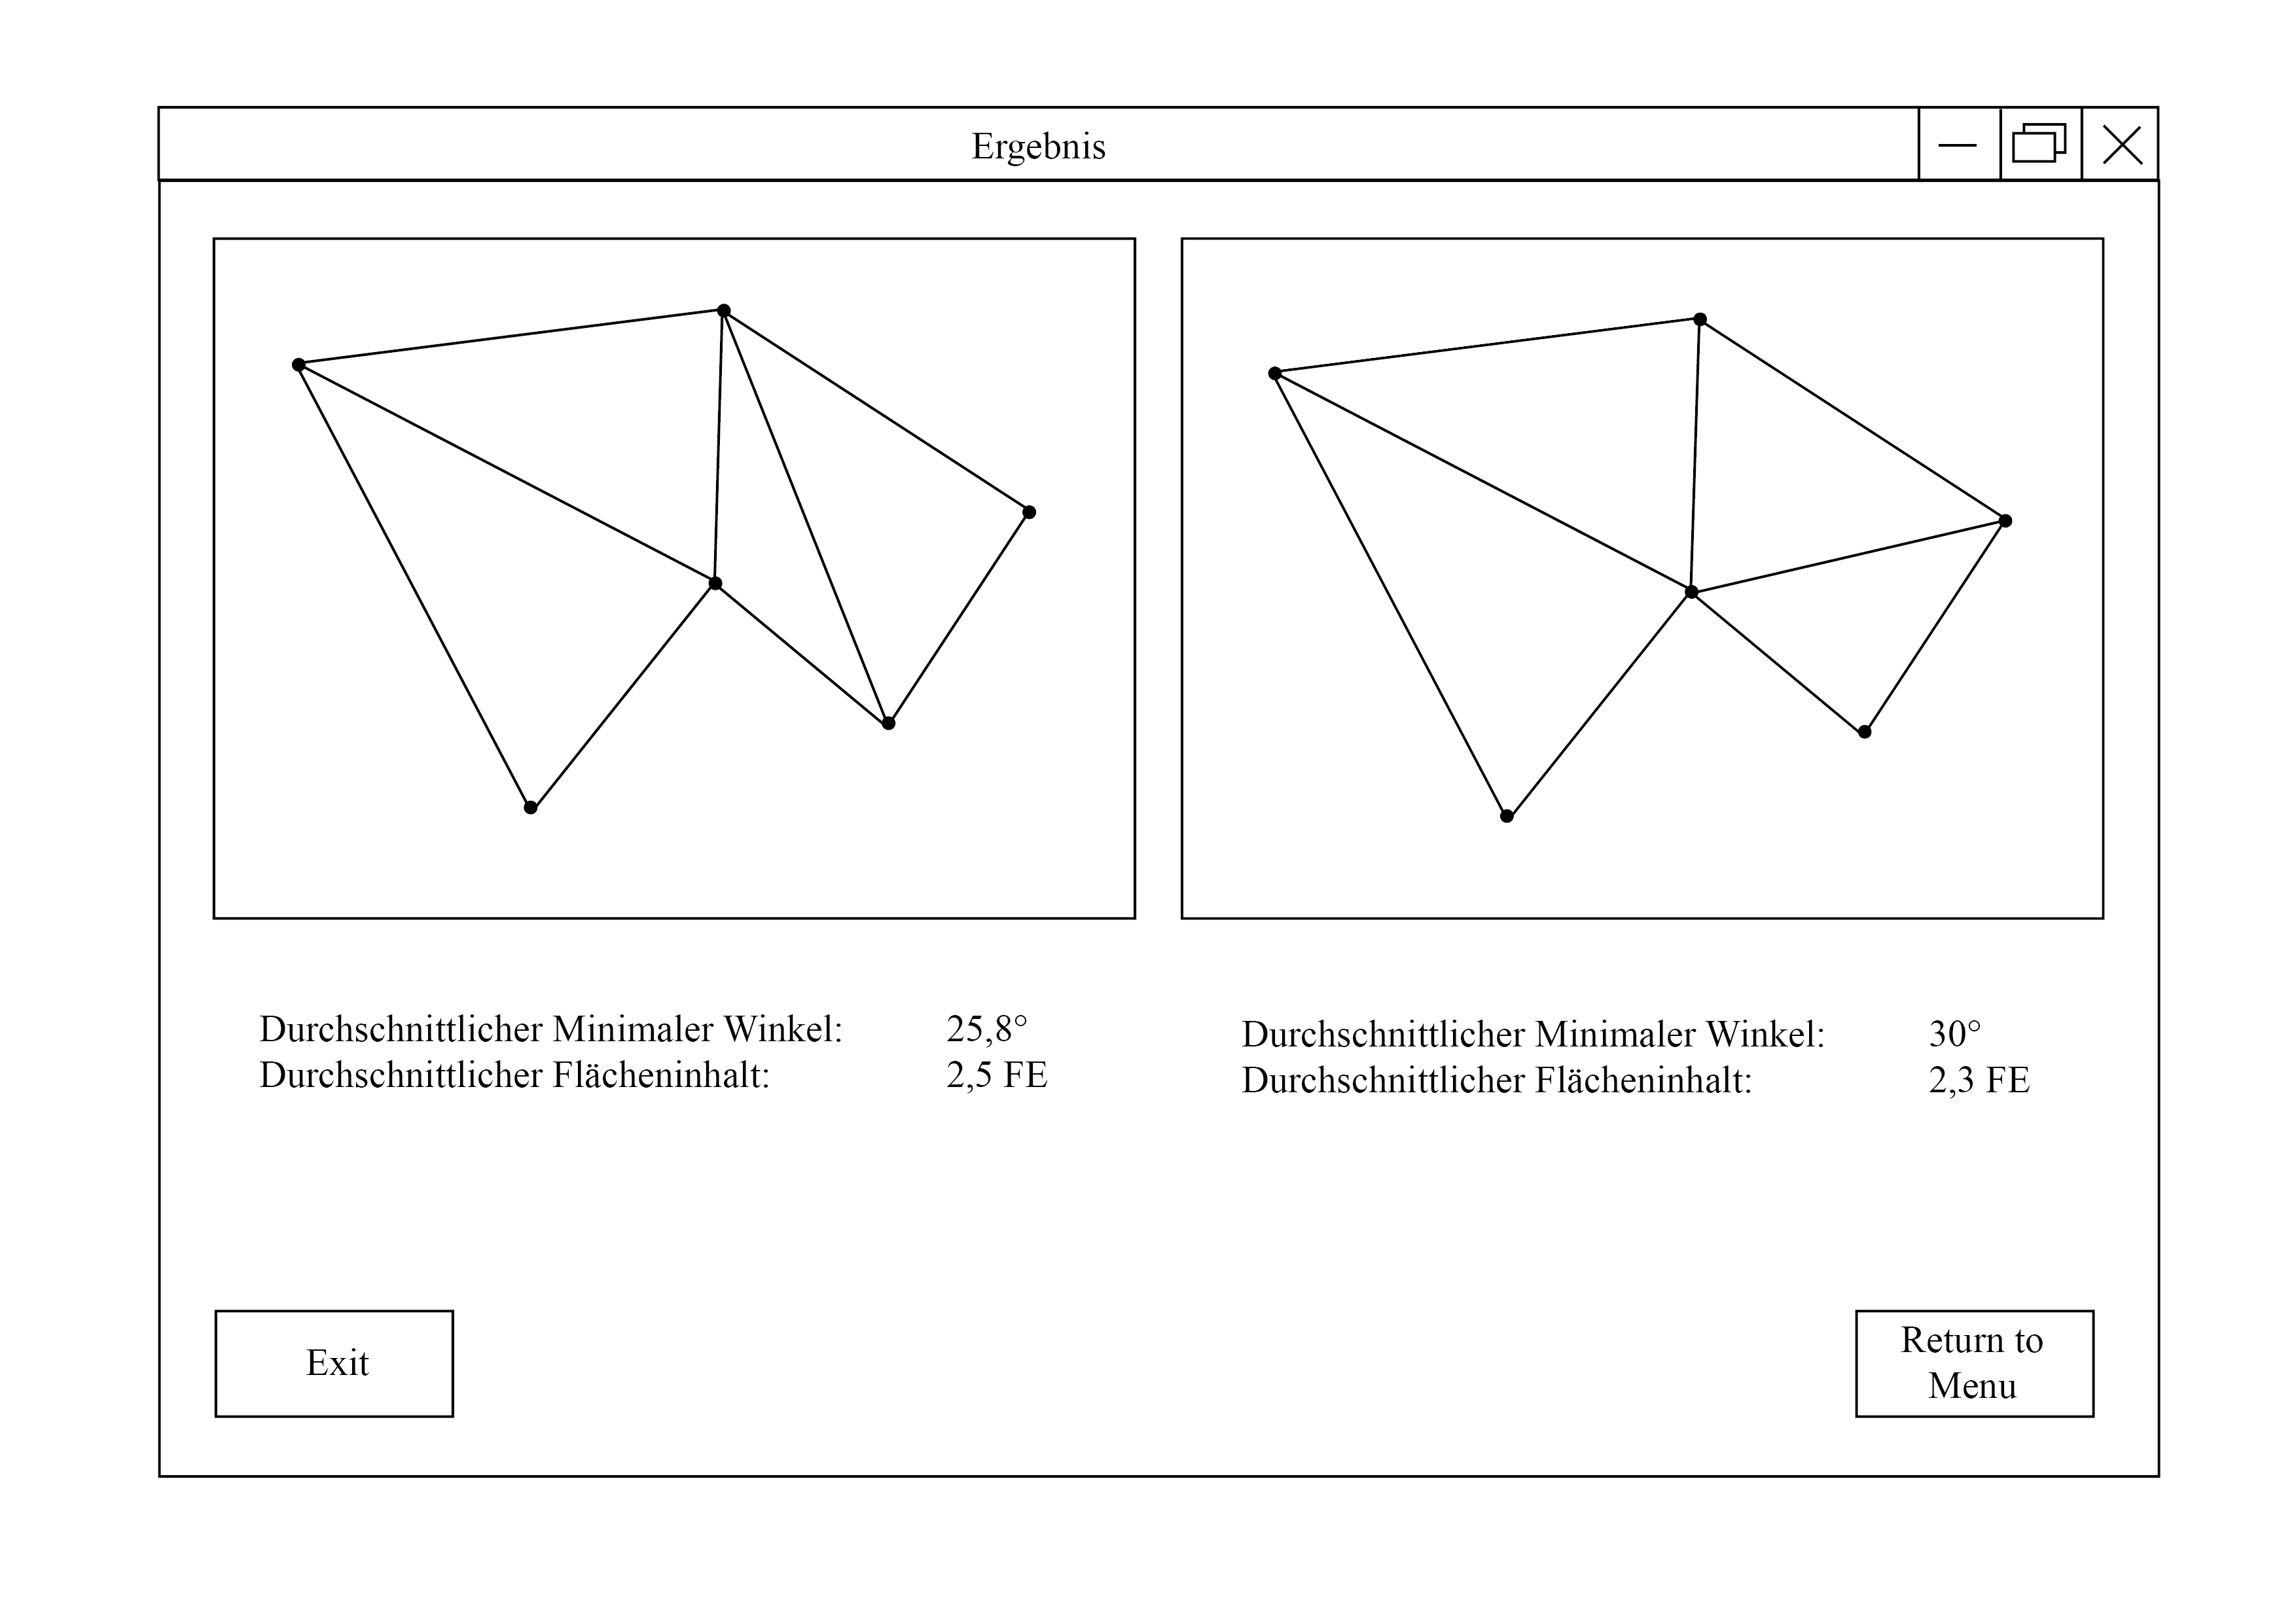
\includegraphics[width=1\textwidth]{bilder/ergebnis_vergleich.png}
    \caption[Entwurf Ergebnisseite mit Vergleichsfenster]{Ergebnisseite mit Vergleichsfenster, welches die optimale Zerleguzng des Polygons darstellt. Darunter Metadaten über die Zerlegungen.}
    \label{fig:ergebnis_vergleich}
\end{figure}

\subsubsection{Finalentwurf}
Der finale Entwurf setzt sich aus den besten oben angeführten Entwürfen zusammen. In Papierform umfasste er noch keine Farben oder ähnliches. Diese wurden erst in der eigentlichen Implementierung hinzugefügt, um das \ac{gui} noch weiter zu verbessern.
In seiner Gänze umfasst der Finalentwurf also das Menü, in welchem die Optionen inklusive sind, die Iterationsseite sowie die Ergebnisseite mit Vergleichsfenster. Die Übergänge zwischen den einzelnen Seiten wird wie in den jeweiligen Abschnitten beschriben geregelt.


\subsection{GUI und Pages}
Wie bereits in Kapitel 4.2.6 beschrieben, besteht das \ac{gui} aus drei Teilen. Diese werden durch einen Aufzählungstypen \lstinline{enum Page} dargestellt. Dieser besitzt drei Ausprägungen, wie im folgenden zu sehen, welche zusätzlich eigene Felder für die weitere 
Implementierung der Funktionalitäten besitzen. Dieses Struct wird in der \lstinline{main.rs} deklariert, sowie auch die anderen in diesem Abschnitt besprochenen Komponenten des Codes.

\begin{lstlisting}[language=C]
enum Page {
    Menu { 
        tools: Tools,
        progset: ProgramSettings,
        draw_panel: DrawPanel,
        confirm_button: button::State,
        undo_buffer: Vec<PageMessage>,
        action_buffer: Vec<PageMessage>,
        undo_performed: bool,
        dark_mode: bool,
    },
    Iteration {
        preview_panel: PreviewPanel,
        prevoius_button: button::State,
        next_button: button::State,
        end_button: button::State,
        dark_mode: bool,
        current_step: usize,
        
    },
    Result {
        result_panel: ResultPanel,
        repeat_button: button::State,
        exit_button: button::State,
        dark_mode: bool,
    },
}    
\end{lstlisting}

Auf jede dieser Ausprägungen wird in den folgenden Kapiteln gesondert eingegangen.
Als übergeordneten Datentyp existiert das \lstinline{struct Pages}. 
Es besitzt zwei Felder. Zum einen einen Vektor aus allen Seiten, welche Ausprägungen des \lstinline{enum Page} sind.
Zusätzlich gibt es noch den Zähler  \lstinline{current_page: usize} als Index für den eben beschriebenen Vektor. Er wird später verwendet, um
von einer Seite des Programms zur nächsten zu wechseln.

\begin{lstlisting}[language=C]
    struct Pages {
        pages: Vec<Page>,
        current_page: usize,
    }
\end{lstlisting}

Das \lstinline{struct Pages} erhält eine Implementierung mit verschiedenen Funktionen mit dem nachfolgenden Aufruf.
Die Funktionen sollen an dieser Stelle in vollständigem Umfang aufgeführt werden. Eine namentliche Erwähnung soll hier genügen. 
Nur auf die \lstinline{fn new()} soll einmal genauer eingegangen werden, damit sie exemplarisch für alle weiteren ähnlichen Funktionen erklärt wird.
Wichtig für die Funktionalität des Programms ist vor allem, dass \lstinline{current_page} mit \lstinline{0} initialisiert wird. Das ist gleichbedeutend mit dem Setzen der 
Startseite auf \lstinline{Page::Menu}.

\begin{lstlisting}[language=C]
    impl Pages {
        fn new() -> Pages { ... }
        fn update(&mut self, msg: PageMessage, ) { ... }
        fn view(&mut self) -> Element<PageMessage> { ... }
        fn advance(&mut self) { ... }
        fn return_to_menu(&mut self) { ... }
        fn can_continue(&self) -> bool { ... }
        fn title(&self) -> &str { ... }
    }
\end{lstlisting}

Mittels der \lstinline{fn new()} wird, bei einer Initialisierung einer Variable vom Typ \lstinline{Pages}, die Standardbelegung aller Felder dieses structs festgelegt. 
Dies geschieht beispielsweise beim Start des Programms. Die Datentypen, welche hier zugewiesen werden,
werden an anderer Stelle noch Erwähnung finden, wenn sie eine zentralere Rolle spielen.

Noch ist das Programm allerdings nicht lauffähig. Dazu fehlen noch drei wichtige Bestandteile. Als erstes das \lstinline{struct Gui}. Dieses umfasst zwei Felde, einmal 
\lstinline{pages: Pages} und \lstinline{dark_mod: bool}. Des weiteren wird für dieses Struct eine Implementierung einer \lstinline{iced::Sandbox} vorgenommen.
Die \lstinline{Sandbox} ist ein Applikationstyp aus der Iced-Bibliothek, welcher ein Programm mit \ac{gui} erzeugt, jedoch keine asynchronen Aktionen unterstützt. Hierfür müsste man
eine \lstinline{iced::Application} nutzen, was für einfache Anwendungen, wie diese Arbeit, nicht notwendig ist. Eine solche Implementierung sieht wie folgt aus:

\begin{lstlisting}[language=C]
    impl Sandbox for Gui {
        type Message = Message;

        fn new() -> Gui { ... }
        fn title(&self) -> String { ... }
        fn update(&mut self, event: Message) { ... }
        fn view(&mut self) -> Element<Message> { ... }
    }
\end{lstlisting}

Zuerst wird eine Typendefinition für \lstinline{Message} durchgeführt. Diese ist wichtig für zwei der vier obligatorischen Funktionen einer \lstinline{Sandbox}, denn 
mittels Nachrichten werden alle Rückmeldungen zu Nutzerinteraktionen abgebildet. Die \lstinline{fn new()} weißt den Feldern, wie bereits beschrieben, Standardwerte zu.

Die \lstinline{fn title(&self)} setzt den Text, welcher oben über einer Seite des Programms im Header angezeigt wird. Dieser wird je nach dem, welche Seite aktiv ist,
festgelegt. Dafür findet sich in der Implementierung \lstinline{impl Page} eine Funktion mit gleichem Namen. Diese ist nachfolgend abgebildet.

\begin{lstlisting}
  
    impl<'a> Page {
        
        fn title(&self) -> &str {
            match self {
                Page::Menu { .. } => 
                    "Triangulation for Polygons - Menu",
                Page::Iteration { .. } => 
                    "Triangulation for Polygons 
                        - Algorithm Iteration",
                Page::Result { .. } => 
                    "Triangulation for Polygons - Result",
            }
        }
    }

\end{lstlisting}

Die \lstinline{fn update(&mut self, event: Message)} hat die Aufgabe, die Übergänge zwischen den einzelnen Seiten zu bewerkstelligen und die jeweilige Update-Funktion 
der einzelnen Pages aufzurufen. Für die Übergänge werden bestimmte Nachrichten abgefangen, welche von Buttons auf den jeweiligen Seiten generiert werden. Dazu aber in späteren Kapiteln mehr.

Zu guter Letzt gibt es noch die \lstinline{fn view(&mut self)}. Diese ist für alle visuellen Aspekte des Programms zuständig. Hier wird das übergeordnete Layout der Pages festgelegt und die 
zur aktiven Page gehörende View-Funktion aufgerufen. Diese legt dann das spezielle Layout jeder Seite fest.

Die Nachrichten, welche während der Laufzeit des Programms von den einzelnen Interaktionselementen generiert und ausgegeben werden, müssen behandelt werden, um alle Funktionalitäten auch bei Aufruf auszuführen.
Dafür hat der der Struct \lstinline{Page} ebenfalls eine Funktion \lstinline{fn update()}. Diese besteht aus einem großen \lstinline{match}-Statement, welches für jeden auftretenden Nachrichtentypen vom Typ \lstinline{PageMessage} die gewünschten 
Aktionen durchführt. Dieses wird in späteren Kapiteln in Teilen betrachtet werden. Hier seinen einmal alle Nachrichtentypen angeführt. Diese sind in der Datei \lstinline{message.rs} definiert.

\begin{lstlisting}
    pub enum PageMessage {
        //Messegaes needed for inteactions on the menu page
        
        //Options
        AlgorithmSelected(Algorithm),
        HeuristicSelected(Heuristic),
        EdgeSwappingToggled(bool),
        StepTrigToggled(bool),
        DarkModeToggled(bool),
    
        //Drawing Tools
        DrawPressed,
        DrawHolePressed,
        UndoPressed,
        RedoPressed,
        ClearPressed, //Opens Popup
        PopUpClosed, //Closes PopUp
        AddPoint(Point),
        ConfirmPressed,
        ClearAll,
        RejectClear,
        
        //Messages for interactions on the iteration page
        PreviousPressed,
        NextPressed,
        EndPressed,
    
        //Messages for interactions on the result page
        ExitPressed,
        RepeatPressed,
    }
\end{lstlisting}

Das zweite noch fehlende Element, um das Programm lauffähig zu machen, ist die \lstinline{fn main()}. Diese ist das Kernstück eines jeden Rust-Programms. Sie ist so lange aktiv, bis das Programm beendet wird.
Sie hat in diesem Fall die Funktion, die \lstinline{Sandbox} zu starten und ablaufen zu lassen. Dazu können der \lstinline{fn Gui::run()}, welche durch die Implementierung der \lstinline{Sandbox} hinzugefügt wurde, verschiedene 
Einstellungsmöglichkeiten vom Typ \lstinline{Settings} übergeben werden. Darunter sind beispielsweise die Höhe und Breite des Programmfensters, ob dieses skalierbar sein soll und anderes. Alles was man nicht per Hand festlegt,
wird durch \lstinline{..Settings::default()} auf einen Standardwert gesetzt. Das Ganze sieht dann wie folgt aus: 

\begin{lstlisting}[language=C]
  
    pub fn main() -> iced::Result {

        Gui::run(Settings {
            antialiasing: true,
            window: window::Settings {
                resizable: false,
                position: Position::Centered,
                size: (1280, 720),
                ..window::Settings::default()
            },
            ..Settings::default()
        })
    }

\end{lstlisting}

Die letzte wichtige Komponente eines Rust-Projekts ist die \lstinline{Cargo.toml} Datei. Sie beinhaltet alle relevanten Informationen für den Compiler, wie zum Beispiel die 
Dependencies. Für dieses Projekt sieht es folgendermaßen aus:

\begin{lstlisting}
  
    [package]
        name = "src"
        version = "0.1.0"
        author = "Christoph Pooch"
        edition = "2021"

    [dependencies]
        iced = {version = "0.4", features = ["canvas"]}
        iced_aw = { version = "0.2", default-features = false, features = ["card"]}
        num-traits = "0.2"
    [[bin]]
        name = "src"
        path = "main.rs"

\end{lstlisting}

Das Programm kann nun mittels des Befehls \lstinline{cargo run} in der Kommandozeile ausgeführt werden.

\subsubsection{Page - Menu}
Wie bereits im Kapitel 4.2.6 zusehen war, setzt sich das Menü aus drei großen Bereichen zusammen, der Zeichenfläche, den Zeichenwerkzeugen und den Optionen. \linebreak

\textbf{Zeichenfläche}\linebreak
Über die Zeichenfläche, welche der zentralste Bestandteil des Menüs ist, wird das Polygon eingegeben, welches im weiteren Verlauf dann mittels des gewählten Algorithmus zerlegt werden soll.
Hierfür besitzt die \lstinline{Page::Menu} ein Feld \lstinline{draw_panel: DrawPanel}. Dieser Struct wird in der Datei \lstinline{draw_panel.rs} definiert und mehrere hat Felder, wie nachfolgend zu sehen. 
Davon ist \lstinline{polygon: DrawState} der Teil, welcher, zusammen mit dem Vektor \lstinline{vertices: Vec<Point>} als Eingabespeicher, die Zeichenfunktionalität umsetzt. Man kann sich den \lstinline{DrawState} als Zustandsautomaten 
vorstellen, welcher drei Zustände vom Typ \lstinline{pending: Option<Pending>} ( \lstinline{None, WaitNxtInput, ClipToStartVertex} ) und einen Cache für die Zeichenoperationen des Renderers besitzt. 

\begin{lstlisting}
    pub struct DrawPanel {
        pub polygon: DrawState,
        pub vertices: Vec<Point>,
        pub panel_width: u16,
        pub panel_height: u16,
        pub closed: bool,
        pub ignore_input: bool,}
\end{lstlisting}

Um nun einen Mausklick über dem Zeichenfenster abzufangen, wird vor jedem Zeichenvorgang eine Überprüfung durchgeführt, ob der Input gesperrt wurde. Das geschieht, wenn 
das Zeichenwerkzeug \emph{Draw} nicht aktiviert ist, damit keine ungewollten Eingaben entstehen. Wenn das nicht der Fall ist, also die Variable \lstinline{ignore_input: bool} auf \lstinline{false} gesetzt ist, dann 
wird eine zweite Überprüfung durchgeführt. Hierbei wird abgefragt, ob sich der Mauszeiger in den Grenzen des Zeichenfeldes befindet und eine relative Position bezogen auf das Zeichenfeldkoordinatensystem ausgegeben.

\begin{lstlisting}
    let cursor_position =
        if self.ignore_input {
            return (event::Status::Ignored, None);
        }
        else if let Some(position) = cursor.position_in(&bounds){
            position
        } else {
            return (event::Status::Ignored, None);
        };

\end{lstlisting}

Diese Information wird nun an den Zustandsautomat, der mittels einem \lstinline{match}-Statement umgesetzt wurde, übergeben. Er überprüft, ob ein Mausklick stattgefunden hat, und führt dann einen Zustandsübergang aus, wenn das geschehen ist.
Dabei wird bei Programmstart im Zustand \lstinline{None} begonnen. Nach der ersten Eingabe bleibt der Automat solange im Zustand \lstinline{WaitNxtInput} und gibt einen Nachricht vom Typ \lstinline{PageMessage::AddPoint(Point)} aus, bis sich der Mauszeiger in einem 
kleinen Bereich um den zuerst eingegebenen Eckpunkt des Polygons befindet. 
In diesem Fall geht er in den Zustand \lstinline{ClipToStartVertex} über. Hier wird kein Punkt hinzugefügt, sondern das Polygon mit einer letzten Kante geschlossen. Dazu wird die Variable \lstinline{closed: bool} des Zeichenfeldes auf \lstinline{true} 
gesetzt. 
Die angesprochene Nachricht wird, wie alle Nachrichten vom Typ \lstinline{PageMessage}, in der Funktion \lstinline{fn update()} des Structs \lstinline{Page} behandelt. Dies sieht folgendermaßen aus:

\begin{lstlisting}
    fn update(&mut self, msg: PageMessage) {
        match msg {
            PageMessage::AddPoint(vertex) => {
                if let Page::Menu { draw_panel, 
                    tools, action_buffer, undo_performed, 
                    undo_buffer,.. } = self {

                    tools.clear_active = true;
                    tools.undo_active = true;
                    
                    if *undo_performed {
                        undo_buffer.clear();
                        tools.redo_active = false;
                    }

                    Page::push_vertex_to_buffer(vertex, 
                        &mut draw_panel.vertices);            
                    
                    draw_panel.polygon.request_redraw();

                    action_buffer.push(
                        PageMessage::AddPoint(vertex));     
                }}
        ...
        }}
\end{lstlisting}
Es werden zunächst einmal zwei Buttons der nachfolgend besprochenen Zeichenwerkzeuge aktiviert - der \emph{Clear-} und der \emph{Undo-Button}. Dann wird eine Überprüfung durchgeführt, ob zuvor eine \emph{Undo-Aktion} 
durchgeführt wurde. Das wird später noch einmal thematisiert. Eben dafür wird auch die Nachricht selbst am Ende des Codeblocks noch in einen Buffer geschoben.
Die zentrale Aufgabe dieses Aufrufs ist jedoch das Hinzufügen des in der Nachricht angegebenen Punktes. Das geschieht mittels der Funktion \lstinline{fn push_vertex_to_buffer()}. Ihr wird 
der Punkt sowie der Buffer übergeben, in welchen er eingefügt werden soll. In diesem Fall ist es der Vektor \lstinline{draw_panel.vertices}. Danach wird noch der Cache des Renderers zurückgesetzt, wodurch alle Inhalte auf dem 
Zeichenfenster neu gezeichnet werden.\linebreak

\begin{figure}[h]
    \centering
    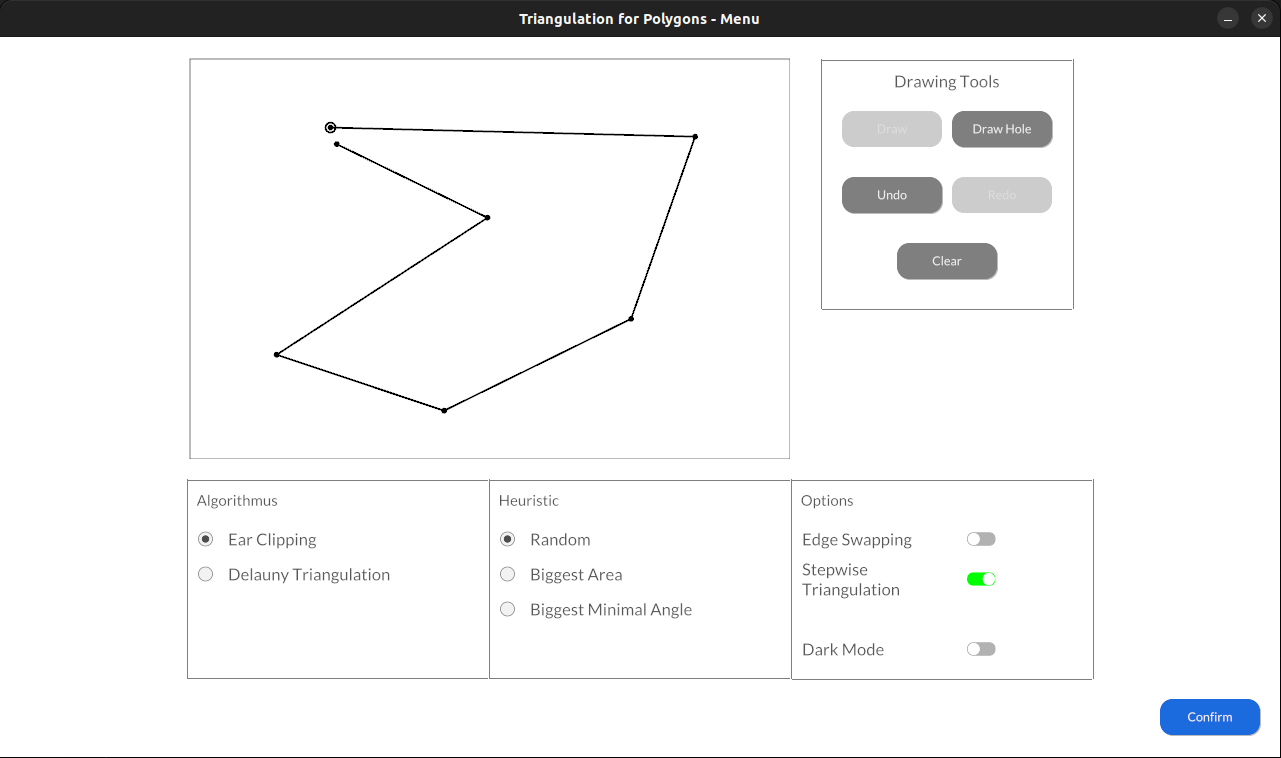
\includegraphics[width=0.8\textwidth]{bilder/menu.png}
    \caption[Menüseite der Anwendung]{Menüseite der Anwendung als Bildschirmfoto}
    
\end{figure}

\textbf{Zeichenwerkzeuge}\linebreak
Der zweite Bereich des Menüs, welcher eng mit dem Zeichenfenster verbunden ist, sind die Zeichenwerkzeuge. Dafür wurde ein neuer Struct in der Datei \lstinline{tools.rs} angelegt.  Bei den Zeichenwerkzeug handelt es sich im Wesentlichen um Buttons, welche verschiedene Funktionalitäten aktivieren.
Es gibt fünf solcher Buttons, welche jeder eine eigene Aufgabe erfüllen. Namentlich sind das der \emph{Draw-}, der \emph{Draw Hole-}, der \emph{Undo-}, der \emph{Redo-} und der \emph{Clear-}Button. Auf jeden davon wird im folgenden einmal gesondert eingegangen.
Der Tool-Struct umfasst also die Zustände der Buttons sowie einigen Boolean-Variablen, welche angeben, ob ein Button aktiv ist oder nicht. Des weiteren umfasst die Implementierung dieses Structs die Funktion \lstinline{pub fn tool_menu()}, welche das Layout der Zeichenwerkzeuge festlegt.
Zu besseren Übersicht für den Nutzer wurden diese fünf Buttons in einer umrahmten Gruppe rechts vom Zeichenfeld angeordnet.

Bevor nun auf die einzelnen Buttons und deren Funktionalität eingegangen wird, soll hier kurz beschrieben sein, wie ein \lstinline{iced::button} überhaupt aufgebaut ist. 
Wie angedeutet, ist ein Button ein Element aus der Iced-Bibliothek. Es besitzt einen Zustand und ein Label, also eine Beschriftung. Zusätzlich gibt es noch eine Nachricht, welche beim Drücken des Buttons ausgelöst wird, und neben vielen weiteren Einstellungen wie Breite und Höhe auch noch einen 
Stil, welcher mittels eines \lstinline{StyleSheets} festgelegt werden kann. Eine Nachricht wird durch den Befehl \lstinline{mybutton.on_press(Message)} an den Button gebunden. 
Zu Stilen ist im Kapitel 4.3.4 mehr beschrieben. Hier einmal der grundsätzliche Aufruf eines neuen Buttons:


\begin{lstlisting}
    use iced::{Button, button, Text};
    neuer_button = Button::new(button::State::new(), 
                   Text::new("Beschriftung"))
                   .on_press(Message).style(ButtonStyle);
\end{lstlisting}

Das Layout, welches in der Funktion \lstinline{pub fn tool_menu()} festgelegt wurde, ist im nachfolgenden Bild noch einmal als Ausschnitt aus dem vollständigen Menü zusehen.
\linebreak

\textbf{\small{Draw-Button}}\linebreak
Dieser Button hat eine der wichtigsten Funktionen des Programms. Er aktiviert die Eingabe auf dem Zeichenfeld. Standardmäßig ist er aktiv, das heißt, es ist möglich ihn zu drücken. Einmal gedrückt, wird er so lange 
deaktiviert, bis ein anderer Button gedrückt wurde. Während er inaktiv ist, das heiß er gedrückt wurde, kann man nach belieben auf dem Zeichenfeld ein Polygon durch Mausklicks erzeugen. Ist dieses dann geschlossen, wird der 
Input wieder deaktiviert.\linebreak

\textbf{\small{Draw-Hole-Button}}\linebreak
Der \emph{Draw-Hole-Button} soll, wie der \emph{Draw-Button}, den Input auf dem Zeichenfeld erlauben. Anders als bei \emph{Draw} soll hier aber nicht auf dem ganzen Zeichenfeld
gezeichnet werden, sondern nur innerhalb des zuvor gezeichneten Polygons. Es sollen also Löcher zum Polygon hinzugefügt werden. Dies ist zum Zeitpunkt der Abgabe dieser Arbeit noch nicht implementiert, wird aber später hinzugefügt.
%evtl rausstreichen
\linebreak

\textbf{\small{Undo-Button}}\linebreak
Das Rückgängigmachen von Aktionen ist ein wichtiger Aspekt, wenn es um Nutzerfreundlichkeit geht. Daher wurde diese Funktion mittels des \emph{Undo-Buttons} implementiert.
Er wird erst aktiv, wenn bereits mindestens ein Punkt auf dem Zeichenfeld gezeichnet wurde. Wird er gedrückt, so wir der zuletzt gezeichnete Eckpunkt aus dem Vektor \lstinline{draw_panel.vertices}, sowie die Nachricht \lstinline{AddPoint(Point)}
aus dem \lstinline{action_buffer} entfernt. In einen zweiten Buffer, den Vektor \lstinline{undo_buffer}, wird dann eine Kopie dieser entfernten Nachricht eingefügt. Sie enthält auch den gelöschten Punkt.
Dies geschieht, damit er mittels des \emph{Redo-Buttons} wieder hinzugefügt werden kann. Dazu im nachfolgenden Abschnitt mehr. Das Drücken des \emph{Undo-Buttons} löst die Nachricht 
\lstinline{PageMessage::UndoPressed} aus, welche dann in der Funktion \lstinline{fn update()} des Page-Struct behandelt wird. Sollte das Polygon zuvor geschlossen worden sein, dann muss dieser Zustand natürlich wieder aufgehoben werden und der Zustand 
des Zeichenautomaten \lstinline{DarwState} muss wieder auf \lstinline{Pending::WaitNxtInput} gesetzt werden. All das wird in der Update-Funktion umgesetzt. Auch wird eine Flag gesetzt, dass die zuletzt durchgeführte Aktion ein Rückgängigmachen war. Das wir 
für die Redo-Aktion relevant.\linebreak

\textbf{\small{Redo-Button}}\linebreak
Der \emph{Redo-Button} stellt das logische Gegenstück zum \emph{Undo-Button} dar. Aktionen, welche mittels Undo rückgängig gemacht wurden, können hiermit erneut durchgeführt werden. Auch dieser Askept ist für die Nutzerfreundlichkeit sehr wichtig.
Zunächst einmal ist dieser Button aber inaktiv. Erst wenn eine Undo-Aktion durchgeführt wurde, kann der \emph{Redo-Button} gedrückt werden.
Wird der \emph{Redo-Button} betätigt, löst er die Nachricht \lstinline{PageMessage::RedoPressed} aus. Diese führt in der \lstinline{fn update()} des Page-Structs zu verschiedenen Abläufen.
Als erstes wird die letzte Nachricht aus dem \lstinline{undo_buffer} entfernt und wieder in den \lstinline{action_buffer} geschrieben. Der zuvor entfernte Punkt, wird wieder in den dafür vorgesehenen Speicher eingefügt.
Sollte es noch weitere Aktionen geben, welche rückgängig gemacht wurden, dann bleibt der Button aktiv und kann erneut gedrückt werden.

In einem weiteren Fall, außer dem, dass der \lstinline{undo_buffer} leer ist, wird der Button auch deaktiviert. Im Prinzip liegt das auch daran, dass der \lstinline{undo_buffer} geleert wurde, aber auf andere Art.
Das geschieht, wenn nach einem Undo ein Draw passiert ist. Zuvor wurde bei der Undo-Aktion eine Flag gesetzt, welche anzeigt, dass die letzte Aktion rückgängig gemacht wurde. Wird jetzt ein neuer Eckpunkt gezeichnet, 
dann wird der \lstinline{undo_buffer} gelöscht. Das geschieht, damit keinen Punkte, welche gelöscht wurden an falscher Stelle wieder in den Vertex-Buffer eingefügt wird. Im nachfolgenden Bild ist das einmal aufgezeigt.
%Bild falscher Redo
\pagebreak

\begin{figure}[t]
    \centering
    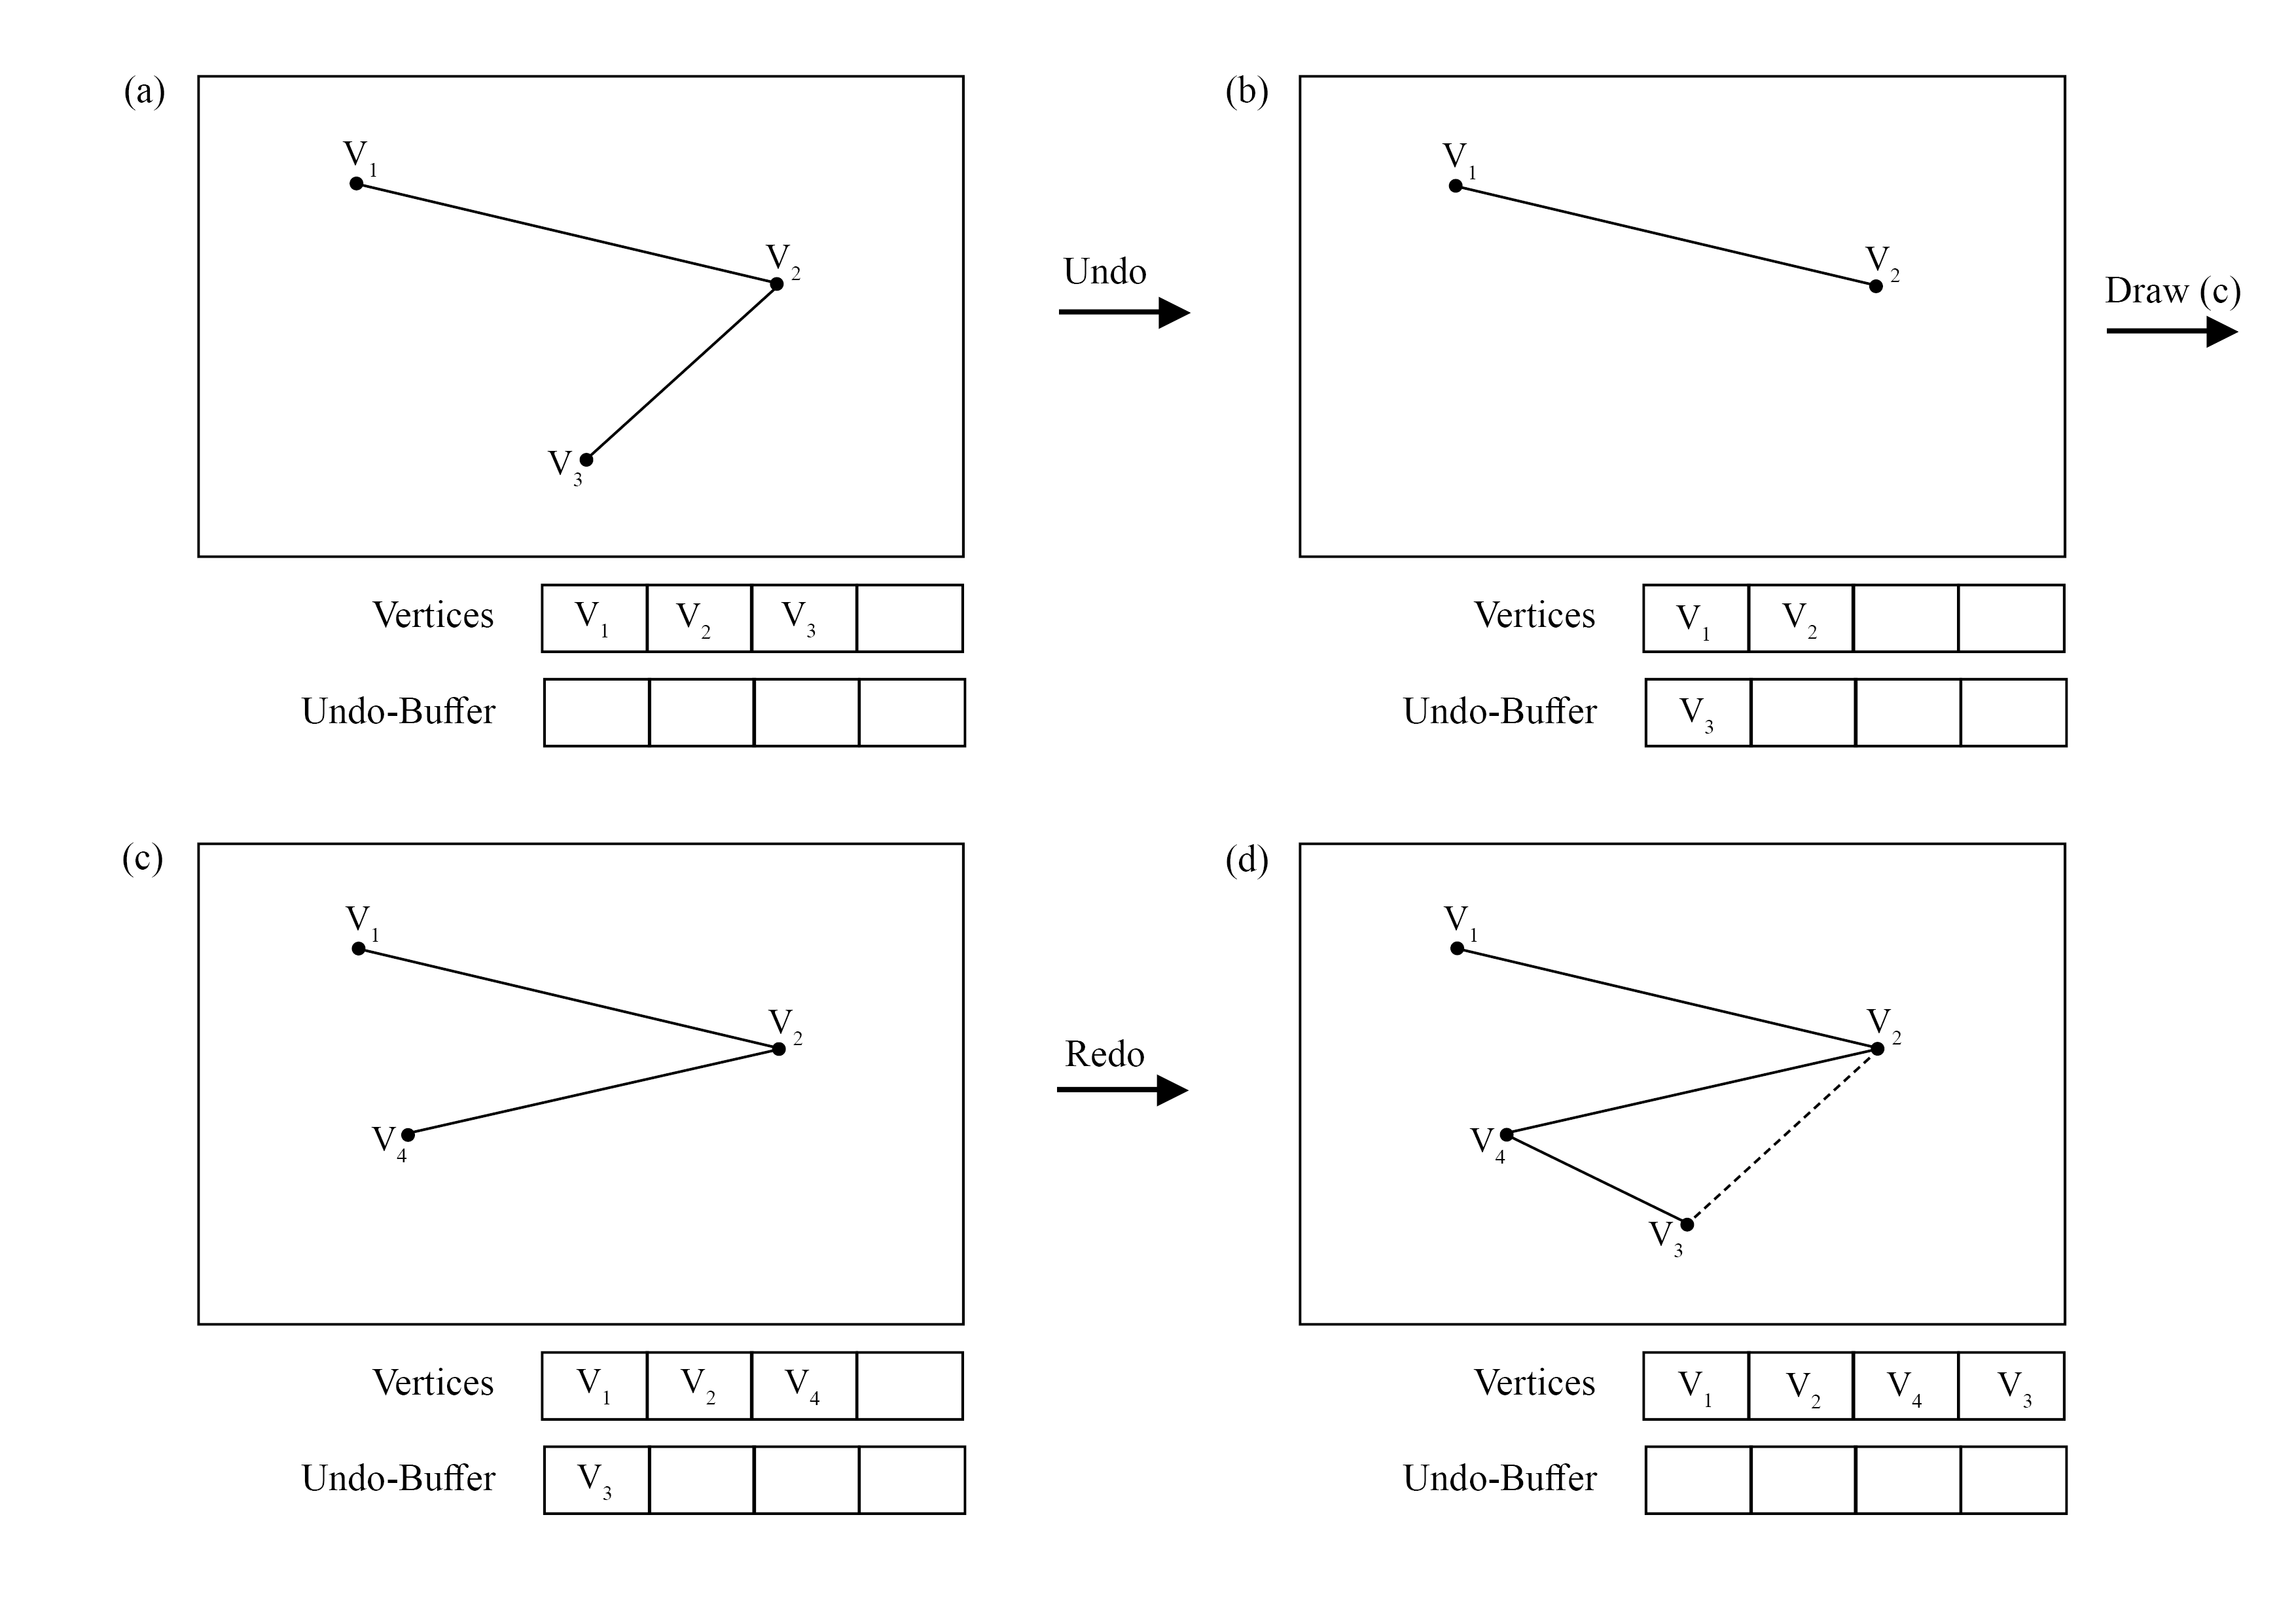
\includegraphics[width=0.7\textwidth]{bilder/falseRedo.png}
    \caption[Fehlerhafter Redo-Vorgang]{Fehlerhafter Redo-Vorgang. Punkt $v_3$ wird entfernt, dann $v_4$ hinzugefügt und später $v_3$ wiederhergestellt.}
\end{figure}
\textbf{\small{Clear-Button}}\linebreak
Dieser Button bildet eine Ausnahme unter den Zeichenwerkzeugen, da seine Funktion eine extra Bestätigung durch ein Dialogfenster benötigt, welches sich dann öffnet, wenn dieser Button gedrückt wurde. 
Dieses Dialogfenster ist kein Element der Iced-Bibliothek. Es gehört zur Bibliothek \lstinline{iced_aw}, welche eine Erweiterung von \lstinline{iced} darstellt und weitere weniger grundlegende \ac{gui}-Elemente umfasst.

\begin{wrapfigure}{h}{0.33\textwidth}
    \centering
    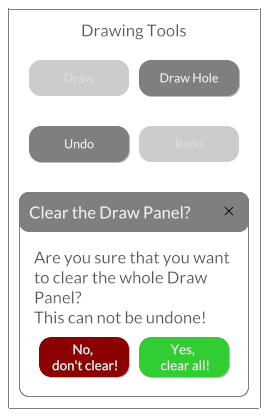
\includegraphics[width=0.3\textwidth]{bilder/clear_dialog.png}
    \caption[Clear-Dialogfenster]{offenes Clear-Diaglogfenster auf der Menüseite}
\end{wrapfigure}

Das verwendete Element ist eine \lstinline{iced_aw::Card}, welche man sich als Fenster im Fenster vorstellen kann. Sie besteht aus Header, Body und Footer und sendet beim Schließen eine Nachricht. 
Im Falle dieser Arbeit ist das \lstinline{PageMessage::PopUpClosed}. Der Body der Karte enthält dabei die Warnung, dass nach der Bestätigung des Löschungsvorganges der gesamte Input auf dem Zeichenfenster gelöscht wird und dies nicht rückgängig gemacht werden kann.
Diese Entscheidung wird mittels eines roten und eines grünen Buttons getroffen. Der rote \emph{Reject-Button} sendet dabei die Nachricht \lstinline{PageMessage::RejectClear} und setzt damit die gleiche Funktionalität um wie die Nachricht \lstinline{PageMessage::PopUpClosed}.
Mit dem grünen \emph{Yes-Clear-Button} wird die Löschung mittels der Nachricht \lstinline{PageMessage::ClearAll} ausgelöst. Beide Buttons schließen die Karte mit dem Dialog und lassen den Ursprünglichen \emph{Clear-Button} wieder erscheinen. 
\linebreak 

\textbf{\large{Optionen}}\linebreak
Der dritte und letzte große Bestandteil der Menü-Seite sind die Optionen. Diese sind ebenfalls noch einmal in drei Teile geteilt, welche optisch, wie auch die Zeichenwerkzeuge, durch einen Rahmen 
abgegrenzt werden. Bei den drei Sektionen handelt es sich um die Auswahl des Algorithmus, die Auswahl der anzuwendenden Heuristik und die weiteren Optionen.
In den ersten beiden Bereichen werden die Auswahlmöglichkeiten durch eine Selektion mittels Radio Buttons abgebildet. Ein Radio Button bzw. eine Radio Button Gruppe hat die Eigenschaft, dass nur eine Option zur gleichen Zeit aktiv sein kann.
Das bedeutet, wenn es drei Möglichkeiten (a), (b) und (c) gibt, dann kann man nur eine der drei, zum Beispiel (b), nicht aber zwei verschiedene, wie etwa (a) und (c), gleichzeitig auswählen.
Die Iced-Bibliothek besitzt eine Implementierung für eben solche Radio Buttons. Man kann sie automatisch aus einem Aufzählungstypen generieren, wenn man für diesen eine Implementierung für \lstinline{impl From<Algorithm> for String} und eine Funktion 
\lstinline{fn all()} bereitstellt. Die Funktion gibt schlichtweg alle Ausprägungen des Aufzählungstypen aus. Die String-Implementierung generiert aus einer gegebenen solchen Ausprägung eine Zeichenkette.
Anhand der Algorithmus-Auswahl sieht das dann in etwa so aus:

\begin{lstlisting}

    pub enum Algorithm {
        EarClipping,
        DelaunyTriangulation,}

    impl<'a> Algorithm {
        pub fn all() -> [Algorithm; 2] {
            [Algorithm::EarClipping,
             Algorithm::DelaunyTriangulation,]
        }}

    impl From<Algorithm> for String {
        fn from(algorithm: Algorithm) -> String {
            String::from(match algorithm {
                Algorithm::EarClipping => "Ear Clipping",
                Algorithm::DelaunyTriangulation => 
                    "Delauny Triangulation",
            })
        }}
\end{lstlisting}
Man bemerke, dass hier zu Beispielzwecken die \ac{dt} als Option aufgeführt ist. Diese ist in der beiliegenden Version des Programms nicht anwählbar. Sie 
ist als Idee der Programmerweiterung im Ausblick noch einmal angeführt.
Die Umsetzung einer automatischen Generierung der Radio Buttons würde dann in etwa so aussehen:

\begin{lstlisting}
    Algorithm::all().iter().cloned().fold(
        Column::new().padding(10).spacing(15),
        |choices, algorithm| {
            choices.push(Radio::new(
                algorithm,
                algorithm,
                selection,
                PageMessage::AlgorithmSelected,
            ).text_size(20).size(15))
        },
    )
\end{lstlisting}

Wie für die Algorithmen in der Datei \lstinline{algorithm.rs} wird nach dem gleichen Schema die selbe Implementierung für die Heuristiken in der Datei \lstinline{heuristc.rs} vorgenommen.
In der Datei \lstinline{program_settings.rs} wir nun der \lstinline{struct ProgramSettings} deklariert, welcher neben  \lstinline{algorithm: Option<Algorithm>} und \lstinline{heuristic: Option<Heuristic>}
auch \lstinline{bools: ProgramSettingsBools} beinhaltet. Dieses Feld umfasst die weiteren Optionen, welche man wahlweise aus- oder anschalten kann. In der finalen Version der Software sind dies zwei Möglichkeiten.
Die Option \emph{Stepwise Triangulation} für die Auswahl, ob der Algorithmus in Schritten oder im Ganzen ausgeführt werden soll, und die Option für den Dark Mode, welcher in Kapitel 4.3.4 beschrieben wird.
Diese Optionen werden durch sogenannte Toggler abgebildet. Ein Toggler hat neben einer Beschriftung auf eine Variable vom Typ Boolean, welchen er je nach seiner eigenen Stellung auf \emph{ein} oder \emph{aus} auf 
\lstinline{true} oder \lstinline{false} setzt. Anhand der Option des Dark Modes sieht das dann so aus:

\begin{lstlisting}
    Toggler::new(
        bools.dark_mode,
        String::from("Dark Mode"),
        PageMessage::DarkModeToggled,
    ).size(15).text_size(20)
\end{lstlisting}\pagebreak

\textbf{\large{Seitenübergang}}\linebreak
Zusetztlich zu den drei großen Bereichen des Menüs gibt es noch ein weiteres Interaktionselement. Dies ist ein Button, welcher unter den Optionen am rechten Rand des Fensters platziert wurde.
Das ist der \emph{Confirm-Button}. Dieser ist, im Gegensatz zu den Zeichenwerkzeugen kein Button mit Sekundärstil sondern ein Primärbutton. Er betsätigt nämlich alle Einstellungen und Eingaben der Menüseite und
regelt den Übergang auf die Iterationsseite. Dazu wird die Nachricht \lstinline{PageMessage::ConfirmPressed} gesendet. Damit das eingegebene Polygon auch auf der nächsten wie auch letzten Seite angezeigt wird, gibt es im Page-Struct
mehrere Funktionen, welche aufgerufen werden, sobald ein Seitenübergang stattfindet. Zuerst einmal muss der Speicher, welcher alle eingegebenen Eckpunkte beinhaltet, ausgelesen werden. Dies geschieht mittels der Funktion 
\lstinline{fn get_vertex_buffer(&mut self)}. Wurde der Buffer ausgelesen, dann muss er in das Koordinatensystem des Anzeigefensters der nächsten Seite konvertiert werden. Das ist notwendig, da alle Anzeigefenster unterschiedliche Größen besitzen.
Das bewerkstelligt die Funktion \lstinline{fn buffer_move_center(buffer: Vec<Point>, offset_x: f32, offset_y: f32)}. Sie erhält als Eingaben neben dem Buffer auch den jeweiligen Offset in x- und y-Richtung
zwischen den beiden Koordinatensystemen. Ist die Transformation geschehen, wird der Buffer mittels der Funktion \lstinline{fn set_vertex_buffer(&mut self, buffer: Vec<Point>)} auf die nächste Seite kopiert.

Für den Übergang zwischen Menü und Iteration genügt das. Für den später noch folgenden Übergang zwischen Iteration und Resultatsseite muss zusätzlich noch der Speicher für die erzeugten Diagonalen übergeben werden.
Dies geschieht nur mittels Kopiervorgang, da keine Koordinaten, sondern Anfangs- und Endpunkte der Strecken gespeichert wurden.

\subsubsection{Page - Iteration}

Die zweite Seite und das eigentliche Kernstück des Programms ist die Iterationsseite. Auf ihr spielt sich die gesamte Visualisierung des algorithmischen Ablaufs ab.
Sie besteht aus nur zwei Teilen. Dem Vorschaufenster und der Navigationsleiste. Den Großteil der Bildfläche nimmt dabei eben jenes Vorschaufenster ein, auf dem das im Menü eingegebene 
Polygon zu sehen ist. Hier werden auch die vom Algorithmus ermittelten Diagonalen eingezeichnet, welche die Triangulation bilden. Diese Einzeichnen geschieht schrittweise, sofern 
im Menü die Option \emph{Stepwise Triangulation} auf aktiv gesetzt wurde. Anderenfalls wird die Iterationsseite übersprungen und sofort die Ergebnisseite aufgerufen.

Das Vorschaufenster wird in der Datei \lstinline{preview.rs} definiert und ist eine vereinfachte Form des Zeichenfensters. Hier ist allerdings die Eingabe standardmäßig deaktiviert, da vom Benutzer keine 
Auswahlen erwartet werden. Nur wenn die Heuristik \emph{Manual Selection} im Menü gewählt wurde, kann der Benutzer per Klick auf ein Dreieck den nächsten Triangulationsschritt bestimmen.
In allen anderen Fällen wird das Dreieck, welches mittels einer Diagonalen gebildet werden soll, automatisch anhand der gewählten Heuristik ausgewählt.

Von einem zum nächsten Iterationsschritt gelangt der Nutzer über einen Button in der Navigationsleiste. Der \emph{Next-Button} erhöhrt den Zähler, welcher den Fortschritt der Triangulation anzeigt, 
und lässt die Anzeige um die neu erzeugte Diagonale erweitern. Es handelt sich hierbei um einen Primärbutton, der dem Nutzer suggerieren soll, dass dies der empfohlene Weg ist, um durch die Triangulation zu navigieren.

Um sich vergangene Iterationsschritte erneut anzegen zu lassen, gibt es den \emph{Previous-Button}, dieser senkt den Fortschrittszähler und zeigt den vorherigen Iterationsschritt auf dem Vorschaufenster an.
Dabei kann man allerdings nicht weiter als bis zum ersten Schritt zurückkehren, da der Button dann deaktiviert wird. Es gibt also keine Möglichkeit, um von der Iterationsseite direkt zur Menüseite zurückzukehren.
Damit das Anzeigen vergangener Schritte nicht als Pflicht empfunden wird, ist der \emph{Previous-Button} im Sekundärstil gehalten.

Hat der Algorithmus alle Schritte durchlaufen, dann wird aus dem \emph{Next-Button} der \emph{End-Button}. Dieser kopiert den Vertex-Buffer wie auch den Diagonalen-Buffer von der Iterationsseite auf die Ergebnisseite 
und sendet die Nachricht \lstinline{PageMessage::EndPressed}, welche von der Update-Funktion des Pages-Structs als Signal zum Übergang auf die Ergebnisseite interpretiert wird. Der \emph{End-Button} ist ebenso wie der 
\emph{Next-Button} ein Primärbutton.

\begin{figure}[h]
    \centering
    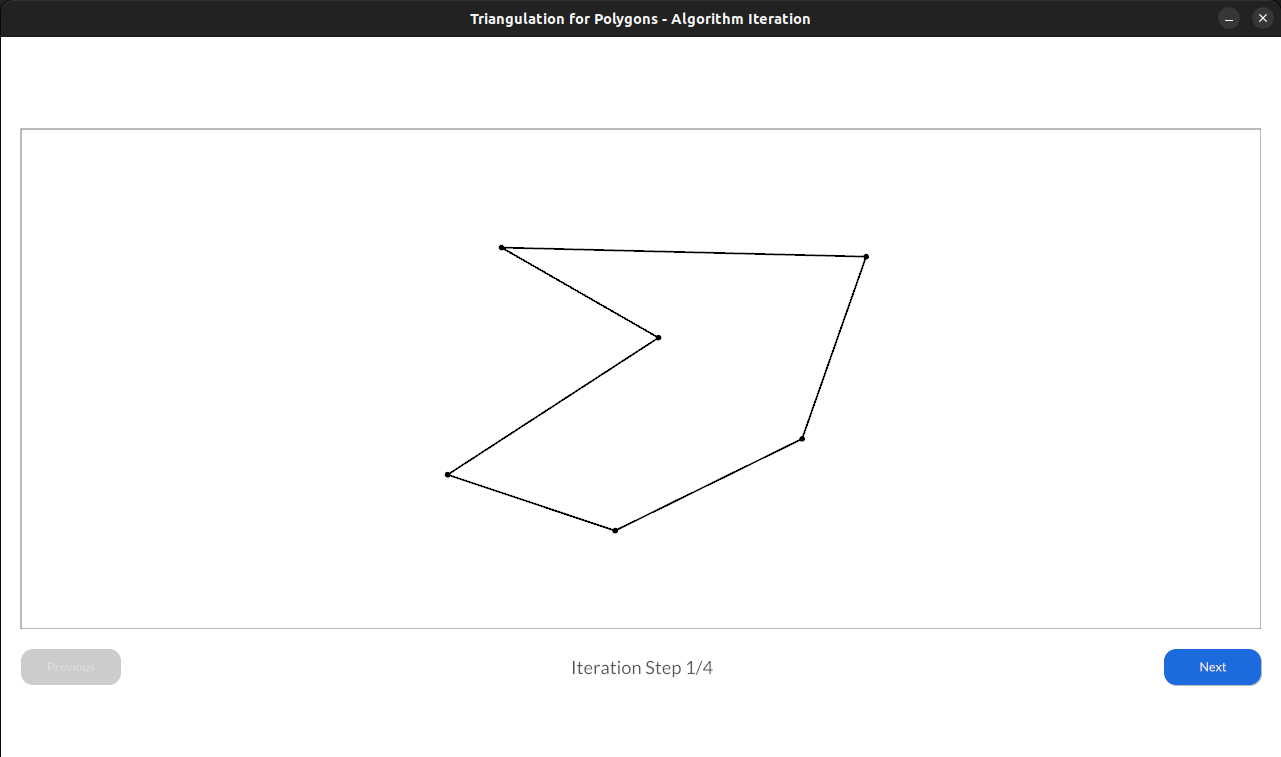
\includegraphics[width=1\textwidth]{bilder/iteration_final.png}
    \caption[Iterationsseite der Anwendung]{Iterationsseite der Anwendung als Bildschirmfoto}
\end{figure}

\subsubsection{Page - Result}

Die Ergebnisseite setzt sich aus zwei Anzeigefenstern mit zugehörigen Informationen zu den abgebildeten Triangulationen und einer Navigationsleiste zusammen.
Dabei ist das linke der beiden gleichgroßen Fenster das jenige, welches die durchlaufene Triangulation zeigt, die auf der Iterationsseite abgebiltet war. Darunter finden sich 
Informationen über das zerlegte Polygon. Namentlich der durchschnittliche Flächeninhalt der Dreiecke und deren durchschnittlicher kleinster Innenwinkel. Außedem wird die Anzahl an Ecken sowie Dreiecken angezeigt.

Das zweite Fenster soll in einer späteren Version eine Vergleichstriangulation, die \ac{dt}, zeigen. Ebenfalls sollen hier die Metadaten der Triangulation aufgezeigt werden.

Die Navigationsleiste besteht aus zwei Buttons. Auf der linken Seite befindet sich der \emph{Exit-Button}, welcher das Programm beendet. Damit der Nutzer weiterhin das Programm benutzen möchte, um weitere Triangulationen durchzuführen,
ist dieser Button im Sekundärstil gehalten.
Dagegen ist der andere Button auf der rechten Seite ein Primärbutton. Seine Beschriftung zeigt \emph{Return to Menu}. Wird er gedrückt, dann wird erneut das Menü aufgerufen. Im Zeichenfenster ist noch das zuvor eingegebene Polygon zu sehen.
Das hat den Zweck, dass der Nutzer mit dem selben Polygon aber anderen Einstellungen eine weitere Triangulation durchführen kann, welche eventuell ein besseres Ergebnis zeigt.
Eine denkbare Funktion wäre es, dass statt der \ac{dt} auf dem zweiten Anzeigefenster die vorangegangene Triangulation angezeigt wird, sofern sich das Polygon nicht verändert hat, welches zerlegt wird.

\begin{figure}[h]
    \centering
    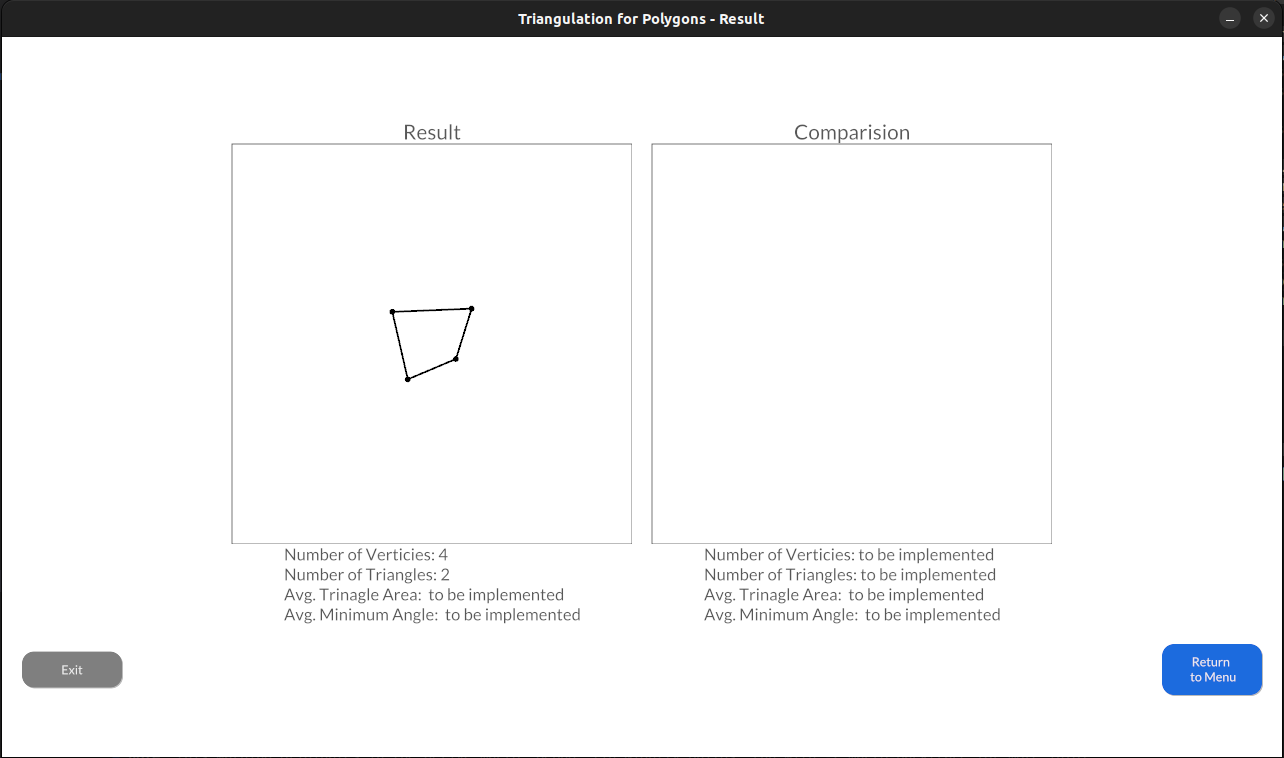
\includegraphics[width=1\textwidth]{bilder/result.png}
    \caption[Ergebnisseite der Anwendung]{Ergebnisseite der Anwendung als Bildschirmfoto}
\end{figure}


\subsubsection{Style und Dark Mode}
Ein großer Aspekt bei der Umsetzung von \ac{gui}s sind Farben. So haben bestimmte Farben für den Menschen bestimmte Bedeutungen - etwa Rot für Gefahr oder Ablehnung.
Dies nutzt man, um dem Benutzer bestimmte Botschaften zu übermitteln. So sind farblich hervorgehobene Buttons zum Beispiel wichtiger als graue. Hierfür müssen diese Farben festgelegt werden.
Das geschieht in der Datei \lstinline{style.rs} mittels der Implementierung von \lstinline{StyleSheets} für verschiedene Aufzählungstypen.
Dabei wird für jedes Interaktionselement wie Buttons, Radio Buttons aber auch für das Fenster selbst ein \lstinline{enum} erstellt, welcher alle verschiedenen Möglichkeiten für Stile des jeweiligen Elements 
umfasst. 

Hier soll einmal exemplarisch gezeigt werden, wie ein solches \lstinline{StyleSheet} für einen \lstinline{iced::container} aussieht. Dieser beinhaltet in jeder View-Funktion den Inhalt einer Seite 
und umfasst derher die Hintergrundfarbe \lstinline{backgroundcolor} und die Schriftfarbe \lstinline{text_color} des Anzeigefensters. 
Zuerst wird im Aufzählungstypen \lstinline{enum WindowStyle} festgelegt, wie viele unterschiedliche Stile ein solcher Container haben kann. 
Danach wird für jeden Stil pro Eigenschaft eine Farbe festgelegt. Alle Eigenschaften, welche dem festgelegten Standard der Iced-Bibliothek folgen sollen, werden mittels 
\lstinline{..Style::default()} abgebildet. So gibt es für Container in dieser Arbeit zwei Stile, wie für die meisten anderen Element auch. Die einzige Ausnahme bilden die Buttons, welche eine rot und grüne, 
sowie eine helle und eine dunkle Variante für Primär- und Sekundärbuttons besitzen. 
Alle anderen Elemente des \ac{gui} haben eine helle und eine dunkle Variante. Der sogenannte \emph{Dark Mode} ist eine weit verbreitete Option für vielerlei Anwendungsprogramme. Da er für einige Nutzer ein obligatorischer Modus ist,
ist er auch in dieser Arbeit implementiert. Er wird wie bereits erwähnt durch einen Toggler im Menü ein- oder ausgeschalten. Dadurch ändern sich alle Stile von der hellen auf die dunkele Variante oder umgekehrt. 
Standardmäßig ist der Dark Mode allerdings aus.

\begin{lstlisting}
    pub enum WindowStyle {
        Light,
        Dark
    }

    impl container::StyleSheet for WindowStyle {
        fn style(&self) -> container::Style {
            container::Style { 
                
                background:  Some(Background::Color(match self {
                    WindowStyle::Light => Color::WHITE,
                    WindowStyle::Dark => Color::from_rgb8(0x57, 0x57, 0x57),
                })),
                text_color: match self {
                    WindowStyle::Light => Some(Color::from_rgb8(0x57, 0x57, 0x57)),
                    WindowStyle::Dark => Some(Color::WHITE),
                },
                ..container::Style::default()
            }}}

\end{lstlisting}

Im nachfolgenden Bild ist der Dark Mode für das Menü als Beispiel angeführt.

\begin{figure}[h]
    \centering
    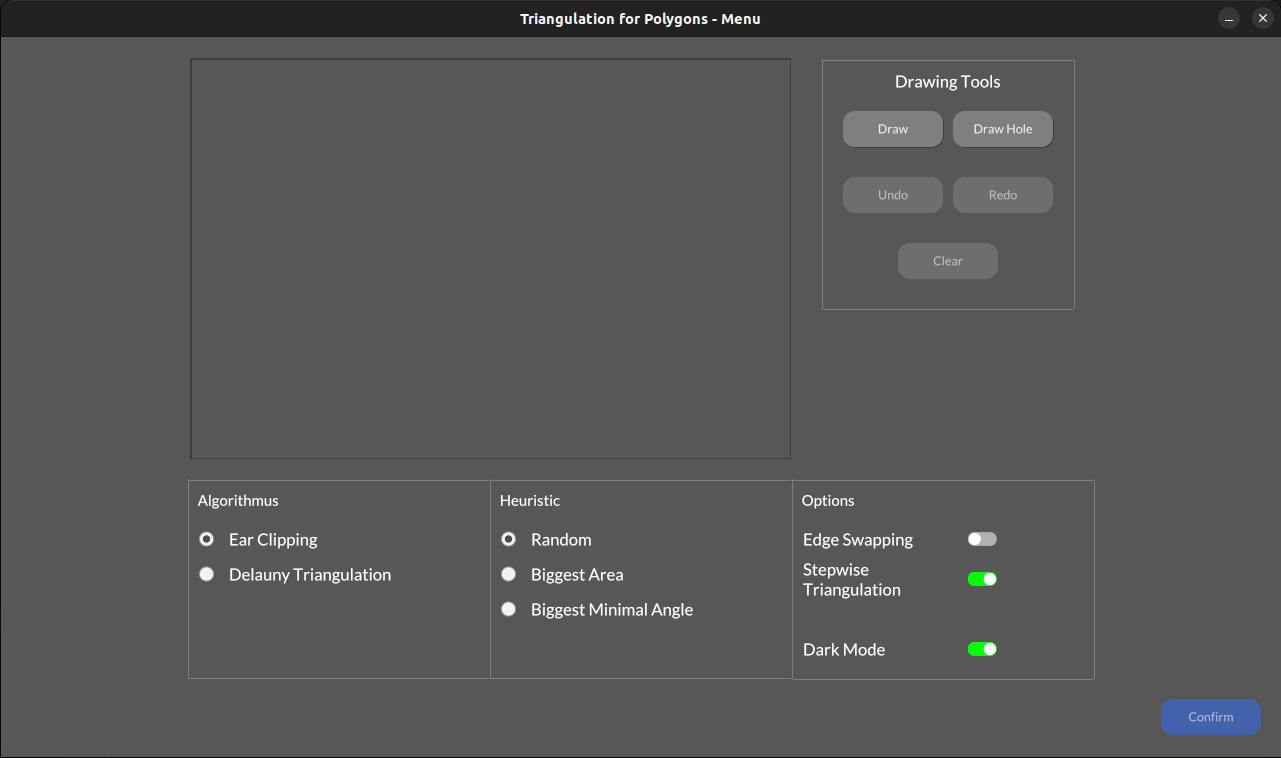
\includegraphics[width=1\textwidth]{bilder/darkmode.png}
    \caption[Menü im Dark Mode]{Das Menü der Anwendung dargestellt mit aktiviertem Dark Mode}
    
\end{figure}
%\subsubsection{Implementierung des Ear-Clipping-Algorithmus}
